\documentclass[12pt, reqno, a4paper]{article}
\usepackage{geometry}        
\geometry{letterpaper} 
\usepackage{graphicx}
\usepackage{caption} 
\usepackage{amssymb}
\usepackage{amsmath}
\usepackage{listings}
\usepackage{color}
\usepackage{chessboard}
\usepackage{fontspec}
\usepackage{etoolbox}
\usepackage{enumitem}
\usepackage{array}
\usepackage{longtable}
\usepackage{metalogo}
\usepackage{tikz}
\usepackage{verbatim}
\usetikzlibrary{arrows,shapes}

\geometry{
	left=30mm,
	right=30mm
}

\newcounter{prob}

\def\problem{\stepcounter{prob}\paragraph{Problem \arabic{prob}}}
\def\solution{\paragraph{Solution}}
\def\algorithm{\mbox{}\\}
\def\sourcecode{\paragraph{Source Code}\leavevmode}
\def\varDescription{\paragraph{Variable Description}\mbox{}}
\def\citeneeded{\textsuperscript{\tiny[citation needed]}}

\newcommand{\chapquote}[2]{\begin{quotation}\begin{center} \textit{#1} \end{center}\end{quotation} \begin{flushright} --- \textbf{#2}\end{flushright}}

\definecolor{codecomment}{rgb}{0.4,0.4,0.4}
\definecolor{codegray}{rgb}{0.5,0.5,0.5}
\definecolor{codestring}{rgb}{0.066,0.5,0.066}
\definecolor{codeblue}{rgb}{0,0.4,0.795}
\definecolor{codelightblue}{rgb}{0.4,0.3,0.8}
\definecolor{codegreen}{rgb}{0,0.4,0.1}
\definecolor{codepink}{rgb}{0.8,0.4,0.3}
\definecolor{codenull}{rgb}{0.6,0.3,0.3}
\definecolor{codepurple}{rgb}{0.6,0.2,0.5}
\definecolor{codeannotation}{rgb}{0.75,0.25,0}

\lstset{
	language=Java,
	aboveskip=3mm,
	belowskip=3mm,
	showstringspaces=false,
	columns=flexible,
	numbers=left,
	morecomment=[l][\color{codeannotation}]{@},
	emph=[1]{return},
	emphstyle=[1]{\color{codegreen}},
	emph=[2]{true, false, null},
	emphstyle=[2]{\color{codepink}},
	emph=[3]{new},
	emphstyle=[3]{\color{codepurple}},
	emph=[4]{for, while, if, else, try, catch, finally},
	emphstyle=[4]{\color{codelightblue}},
	basicstyle={\small\ttfamily\footnotesize},
	numberstyle=\tiny\color{codegray},
	keywordstyle=\color{codeblue},
	commentstyle=\color{codecomment},
	stringstyle=\color{codestring},
	breaklines=true,
	breakatwhitespace=true,
	extendedchars=true,
	tabsize=8
}
\setlist[enumerate]{
	topsep=0mm,
	itemsep=0mm,
	partopsep=0mm,
	parsep=0mm
}

\title{Computer Project}
\author{Satvik Saha}
\begin{document}

	\newfontfamily\Perfograma{Perfograma}
\newfontfamily\JennaSue{Jenna Sue}

\thispagestyle{empty}\addtocounter{page}{-1}
\hspace{0pt}
\begin{center}
\vfill
{\fontsize{36}{28}\tt Computer Project}\\
\vspace{1mm}
{\Perfograma (2017-2019)}
\vfill
{\fontsize{30}{24}\JennaSue Satvik Saha}\\
\vspace{1mm}
{\tt Class: XI B}\\
{\tt Roll number: 24}
\end{center}
\hspace{0pt}
	\thispagestyle{empty}\addtocounter{page}{-1}
\hspace{0pt}
\vfill
\chapquote{``Writing code a computer can understand is science. Writing code other programmers can understand is an art."}{Jason Gorman}
\vfill
\hspace{0pt}

	
\chapquote{``I am rarely happier than when spending an entire day programming my computer to perform automatically a task that would otherwise take me a good ten seconds to do by hand."}{Douglas Adams}

\problem An $n$ digit integer $(a_1a_2\dots a_n)$, where each digit $a_i \in \{0, 1, \dots, 9\}$,
is said to have {\em unique digits} if no digits are repeated, i.e., there is no $i, j$ such that $a_i = a_j$ ($i \neq j$).

Verify whether an inputted number has {\em unique digits}.

\solution The problem involves simply counting the number of occurences of each digit in the given number and checking whether any of them exceed $1$.

\algorithm
{\tt main (number:Integer)}
\begin{enumerate}
	\item	Initialize an integer array {\tt digits} of length {\tt 10}, indexed with integers
			from {\tt [0]} to {\tt [9]} with all elements set to {\tt 0}.
	\item	If {\tt number} exceeds {\tt 0}, proceed.
			Otherwise, jump to (\ref{unique:loopEnd}). \label{unique:loopStart}
	\begin{enumerate}
		\item	Store the last digit\footnote{The last digit of an integer $n$ is simply $n \bmod 10$}
				of {\tt number} in a temporary variable {\tt d}.
		\item	Increment the integer at the {\tt d} index of {\tt digits}.
		\item	If {\tt digits[d]} exceeds {\tt 1}, the number does not have {\em unique digits}. Display a suitable
				message, and {\bf exit}.
		\item	Discard the last digit of {\tt number} by performing an integer division by {\tt 10} and storing
				the result back in {\tt number}.
		\item	Jump to (\ref{unique:loopStart}).
	\end{enumerate}
	\item	The number has {\em unique digits}. Display a suitable message. \label{unique:loopEnd}
	\item	{\bf Exit}
\end{enumerate}

\sourcecode
\lstinputlisting{src/Unique.java}

\varDescription
\begin{longtable} {| >{\ttfamily}p{0.15\linewidth} | >{\ttfamily}p{0.2\linewidth}| p{0.6\linewidth} |}
\hline\multicolumn{3}{|c|}{\tt Unique::main(String[])} 										\\ \hline
long	&	number 	&	The inputted number 													\\ \hline
\hline\multicolumn{3}{|c|}{\tt Unique::isUnique(long)} 										\\ \hline
long	&	number 	&	The number to check for uniqueness									\\ \hline
int[]	&	count	&	The number of occurrences of each digit								\\ \hline
long	&	n		&	Counter, temporarily stores the value of {\tt number}				\\ \hline
int		&	digit	&	The last digit in {\tt n}											\\ \hline
\end{longtable}
	
\chapquote{``Elegance is not a dispensable luxury but a factor that decides between success and failure."}{Edsger W. Dijkstra}

\problem A {\em partition} of a positive integer $n$ is defined as a collection of other positive integers such that
their sum is equal to $n$. Thus, if $(a_1, a_2, \dots, a_k)$ is a partition of $n$,
\begin{equation*}
	n	\;=\;	a_1 + a_2 + \dots + a_k 			\tag{$a_i \in \mathbb{Z}^{+}$}
\end{equation*}

Display every {\em unique partition} of an inputted number.

\solution This problem can be solved elegantly using {\em recursion\footnote{Recursion occurs when a thing is defined in terms of itself or of its type.}}.

\sourcecode
\lstinputlisting{src/Partition.java}
	
\chapquote{``Simplicity is the ultimate sophistication."}{Leonardo da Vinci}

\problem A {\em Caesar cipher} is a type of monoalphabetic substitution cipher in which each letter
in the plaintext is replaced by a letter some fixed number of positions down the alphabet. The positions
are circular, i.e., after reaching $Z$, the position wraps around to $A$. For example, following is some encrypted
text, using a right shift of 5.

\begin{lstlisting}[numbers=none, xleftmargin=.25\textwidth, xrightmargin=.2\textwidth]
Plain:    ABCDEFGHIJKLMNOPQRSTUVWXYZ
Cipher:   FGHIJKLMNOPQRSTUVWXYZABCDE
\end{lstlisting}

Thus, after mapping the alphabet according to the scheme $A\mapsto 0, B\mapsto 1,\dots,Z\mapsto 23$, we can define
an encryption function $E_n$, in which a letter $x$ is shifted rightwards by $n$ as follows.
\begin{equation*}
	E_n(x)	\;=\;	(x + n)	\quad\bmod 26
\end{equation*}

The corresponding decryption function $D_n$ is simply
\begin{equation*}
	D_n(x)	\;=\;	(x - n)	\quad\bmod 26
\end{equation*}

Implement a simple version of a {\em Caesar cipher}, encrypting capitalized plaintext by shifting it by a given value.
Interpret positive shifts as rightwards, negative as leftwards.

\solution This problem can be solved simply by exploiting the fact that Unicode characters are already arranged in order, with successive alphabets encoded by consecutive numbers. In addition, the encryption function can be defined exactly as given in the question --- characters can be converted to their corresponding codes, manipulated by addition of the {\tt shift}, and converted back into alphabetic form.

\algorithm
{\tt main (shift:Integer, plainText:String)}
\begin{enumerate}
	\item	Normalize {\tt plainText} to uppercase.
	\item	Normalize {\tt shift} by replacing it with {\tt shift} $\bmod$ $26$.
	\item	Initialize an empty String {\tt cipherText}.
	\item	Initialize a counter {\tt i} to {\tt 0}.
	\item	If {\tt i} is less than the length of {\tt plainText}, proceed.
			Otherwise, jump to (\ref{cipher:loopEnd}). \label{cipher:loopStart}
	\begin{enumerate}
		\item	Store the character in {\tt plainText} at position {\tt i} in a variable {\tt plain}.
		\item	Initialize an empty character {\tt crypt}.
		\item	If {\tt plain} is not an alphabet, assign {\tt plain} to {\tt crypt} and jump to (\ref{cipher:append}).
		\item	Convert {\tt plain} into a number, such that {\tt A} is mapped to {\tt 0}, {\tt B} to {\tt 1} and so on.
				Store this in a temporary variable {\tt n}.
		\item	Add {\tt shift} to {\tt n}, calculate its least residue modulo $26$\footnote{The set of integers 
				$K = \{0, 1, 2, \dots , n-1\}$ is called the least residue system modulo $n$. The number $k$ such that 
				$k \in K$ and $a \equiv k \pmod{n}$ is called the least residue of $a$ modulo $n$.}, and store the result in {\tt n}.
		\item	Convert {\tt n} back into a character and store the result in {\tt crypt}.
		\item	Append {\tt crypt} to {\tt cipherText}.  \label{cipher:append}
		\item	Increment {\tt i} by {\tt 1} and jump to (\ref{cipher:loopStart}).
	\end{enumerate}
	\item	Display {\tt cipherText}.  \label{cipher:loopEnd}
	\item	{\bf Exit}
\end{enumerate}

\sourcecode
\lstinputlisting{src/CaesarShift.java}

\varDescription
\begin{longtable} {| >{\ttfamily}p{0.15\linewidth} | >{\ttfamily}p{0.2\linewidth}| p{0.6\linewidth} |}
\hline\multicolumn{3}{|c|}{\tt CaesarShift::main(String[])} 									\\ \hline
int		&	shift 		&	The inputted 'shift' 											\\ \hline
String	&	plainText	&	The text to encrypt												\\ \hline
String	&	cipherText	&	The encrypted text												\\ \hline
int		&	i			&	Counter variable, stores the position in {\tt plainText}			\\ \hline
char	&	plain		&	The character to encrypt											\\ \hline
char	&	crypt		&	The encrypted form of {\tt plain}								\\ \hline
\hline\multicolumn{3}{|c|}{\tt CaesarShift::charToNum(char)} 								\\ \hline
char	&	letter	 	&	The character to convert to an integer 							\\ \hline
\hline\multicolumn{3}{|c|}{\tt CaesarShift::numToChar(int)} 									\\ \hline
int		&	number	 	&	The number to convert to a character	 							\\ \hline
\end{longtable}
	
\chapquote{``There are 2 hard problems in computer science: cache invalidation, naming things, and off-by-1 errors."}{Leon Bambrick}

\problem A {\em palindrome} is a sequence of characters which reads the same backwards as well as forwards.
For example, {\tt madam}, {\tt racecar} and {\tt kayak} are words which are palindromes. Similarly, the sentence ``{\tt A man, a plan, a canal -- Panama!}" is also a plaindrome.

Analyze a sentence of input and display all {\em words} which are palindromes. If the entire {\em sentence} is also a palindrome, display it as well.\\

{\em (A word is an unbroken sequence of characters, separated from other words by whitespace. Ignore single letter words such as {\em I} and {\em a}.
Ignore punctuation, numeric digits, whitespace and case while analyzing the entire sentence.)}

\solution The main challenge here is intelligently dividing a {\em sentence} into its component {\em words}. Verifying whether a sequence of characters is a palindrome is fairly simple --- extracting those characters from a string of alphabets, numbers, punctuation and whitespace is not.

The main idea behind isolating words from sentences is to define two {\em markers} --- a {\tt start} to keep track of the boudary between whitespace and letters, and an {\tt end} to mark the boundary between letters and whitespace. In this way, the markers can inch their way along the sentence, isolating words in the process. Managing the order of condition checking and incrementing of counters does require some careful maneuvering in order to avoid any {\em off-by-1 errors\footnote{An off-by-one error often occurs in computer programming when an iterative loop iterates one time too many or too few.}}.

\sourcecode
\lstinputlisting{src/Palindrome.java}
	
\chapquote{``In programming the hard part isn't solving problems, but deciding what problems to solve."}{Paul Graham}

\problem The {\em Sieve of Eratosthenes} is a simple, ancient algorithm for finding all prime numbers up to any given limit.
It does so by iteratively marking as composite the multiples of each prime, starting with the first prime number, $2$.

Implement the {\em Sieve of Eratosthenes} to display primes upto a given limit, as well as the number of primes calculated.

\solution

\sourcecode
\lstinputlisting{src/SieveOfEratosthenes.java}
\lstinputlisting{src/Primes.java}
	
\chapquote{``Any fool can use a computer. Many do."}{Ted Nelson}

\problem Design a simple interface for an examiner which can format and display marks scored by a group
of students in a particular examination. Calculate the percentage scored by each candidate and display the
list of students and percentages in an ASCII bar chart, arranged alphabetically.

\solution This problem calls for a fairly straightforward flow of logic. The main goal is to present the user with a simple way of providing input, along with nicely formatted output.

\algorithm
{\tt main (upperLimit:Integer)}
\begin{enumerate}
	\item	Input the maximum marks allotted for the examination as a floating point.
			Store it as {\tt maxMarks}.
	\item	Input the total number of students whose marks are to be recorded as an integer.
			Store it as {\tt numberOfStudents}.
	\item	Create a new {\tt Marksheet}, pass it {\tt maxMarks}, {\tt numberOfStudents} and assign
			it to {\tt sheet}.
	\item	Initialize an integer counter {\tt i} to {\tt 0};
	\item	If {\tt i} is less than {\tt numberOfStudents}, proceed.
			Otherwise, jump to (\ref{chart:inputLoopEnd}). \label{chart:inputLoopStart}
		\begin{enumerate}
			\item	Input a student's name as a string. Store it as {\tt name}.
			\item	Input the student's marks as a floating point. Store it as {\tt marks}.
			\item	Call {\tt sheet->addMarks(name, marks)}.
			\item	Jump to (\ref{chart:inputLoopStart}).
		\end{enumerate}
	\item	Call {\tt sheet->sortByName()}. \label{chart:inputLoopEnd}
	\item	Call {\tt sheet->displayChart()}.
	\item	Call {\tt sheet->sortMaxScorers()}.
	\item	{\bf Exit}
\end{enumerate}
\vspace{8mm}
{\tt Marksheet (maxMarks:FloatingPoint, numberOfStudents:Integer)}
\begin{enumerate}
	\item	Initialize a string array {\tt names}, indexed with integers from {\tt [0]} to {\tt [numberOfStudents - 1]}.
	\item	Initialize a floating point array {\tt marks}, indexed with integers from {\tt [0]} to 
			{\tt [numberOfStudents - 1]}.
	\item	Initialize an integer counter {\tt lastStudent} to {\tt -1}.
	\item	{\bf Define} the functions: 
	\begin{enumerate}
		\item	{\tt Marksheet::addMarks(name, score)}
		\item	{\tt Marksheet::sortByName()}
		\item	{\tt Marksheet::displayChart()}
		\item	{\tt Marksheet::displayMaxScorers()}
	\end{enumerate}
	\item	{\bf Return} the resultant object.
\end{enumerate}
\vspace{5mm}
{\tt Marksheet::addMarks (name:String, score:FloatingPoint)}
\begin{enumerate}
	\item	Increment {\tt lastStudent} by {\tt 1}.
	\item	Set the {\tt names[lastStudent]} to {\tt name}.
	\item	Set the {\tt marks[lastStudent]} to {\tt score}.
	\item	{\bf Return}
\end{enumerate}
\vspace{5mm}
{\tt Marksheet::sortByName ()}
\begin{enumerate}
	\item	Assign {\tt lastStudent} to {\tt right}.
	\item	If {\tt right} exceeds {\tt 0}, proceed.
			Otherwise, {\bf return}. \label{chart:sortOutLoopStart}
		\begin{enumerate}
			\item	Initialize an integer counter {\tt i} to {\tt 1}.
			\item	If {\tt i} is less than or equal to {\tt right}, proceed.
					Otherwise, jump to (\ref{chart:sortInLoopEnd}). \label{chart:sortInLoopStart}
			\begin{enumerate}
				\item	If {\tt names[i-1]} comes lexicographically after {\tt names[i]}:
				\begin{enumerate}
					\item	Swap the elements at {\tt names[i-1]} and {\tt names[i]}.
					\item	Swap the elements at {\tt marks[i-1]} and {\tt marks[i]}.
				\end{enumerate}
				\item	Jump to (\ref{chart:sortInLoopStart}).
			\end{enumerate}
			\item	Jump to (\ref{chart:sortOutLoopStart}). \label{chart:sortInLoopEnd}
		\end{enumerate}
\end{enumerate}
\vspace{5mm}
{\tt Marksheet::displayChart ()}
\begin{enumerate}
	\item	For every string {\tt name} in {\tt names}:
	\begin{enumerate}
		\item	Calculate the length of the bar in the chart as a fraction of the screen width.
				Store the calculated number of characters to display as {\tt points}.
		\item	Display {\tt name}, a string of suitable characters for the bar of length {\tt points},
				along with the percentage scored.
	\end{enumerate}
	\item	{\bf Return}
\end{enumerate}
\vspace{5mm}
{\tt Marksheet::displayMaxScorers ()}
\begin{enumerate}
	\item	Calculate the maximum floating point in {\tt marks} and store it as {\tt maxScore}.
	\item	For every integer {\tt i} between {\tt 0} and {\tt numberOfStudents} (inclusive, exclusive)
			such that {\tt marks[i]} is equal to the {\tt maxScore}, display {\tt names[i]}.
	\item	{\bf Return}
\end{enumerate}

\clearpage
\sourcecode
\lstinputlisting{src/Marksheet.java}
\lstinputlisting{src/ScoreRecorder.java}

\varDescription
\begin{longtable} {| >{\ttfamily}p{0.16\linewidth} | >{\ttfamily}p{0.2\linewidth}| p{0.6\linewidth} |}
\hline\multicolumn{3}{|c|}{\tt Marksheet} 													\\ \hline
int		&	SCREEN\_WIDTH	 &	Number of characters to use in the display width				\\ \hline
double	& 	maxMarks	&	The maximum marks allotted for the examination					\\ \hline
int		&	numberOf
	\newline Students	&	The number of students whose marks are to be recorded			\\ \hline
int		&	lastStudent	&	The index number of the last student added to the marksheet		\\ \hline
String[]	& names		&	The names of the students										\\ \hline
double[]	& marks		&	The marks of the students										\\ \hline
\hline\multicolumn{3}{|c|}{\tt Marksheet::addMarks(String, double)} 							\\ \hline
String	&	name		&	The name of the student to be added								\\ \hline
double	&	score		&	The marks of the student to be added								\\ \hline
\hline\multicolumn{3}{|c|}{\tt Marksheet::displayChart()} 									\\ \hline
int		&	i			&	Counter variable													\\ \hline
double	&	fraction	&	The fraction on marks scored over the maximum marks				\\ \hline
String	&	name		&	Temporarily stores a formatted version of a student's name		\\ \hline
int		&	points		&	The number of characters to display in the bar chart				\\ \hline
String	&	bar			&	The bar in the chart, along with whitespace padding				\\ \hline
\hline\multicolumn{3}{|c|}{\tt Marksheet::displayMaxScorers()} 								\\ \hline
String	&	maxScorers	&	The list of highest scoring students								\\ \hline
double	&	maxScore	&	The highest score												\\ \hline
int		&	i			&	Counter variable													\\ \hline
\hline\multicolumn{3}{|c|}{\tt Marksheet::sortByName()} 										\\ \hline
int		&	right		&	Counter variable													\\ \hline
int		&	i			&	Counter variable													\\ \hline
\hline\multicolumn{3}{|c|}{\tt Marksheet::getMaxScore()} 									\\ \hline
double	&	max			&	The maximum score in {\tt marks}									\\ \hline
int		&	i			&	Counter variable													\\ \hline
\hline\multicolumn{3}{|c|}{\tt Marksheet::swapRecords(int, int)} 							\\ \hline
int		&	x, y		&	The indices of the records to swap								\\ \hline
String	&	tempName	&	Temporary storage of a name										\\ \hline
double	&	tempMark	&	Temporary storage of a mark										\\ \hline
\hline\multicolumn{3}{|c|}{\tt Marksheet::multiplyString(String, int)} 						\\ \hline
String	&	s			&	The string to multiply											\\ \hline
int		&	n			&	The number of times to multiply {\tt s}							\\ \hline
String	&	out			&	The string containing {\tt n} copies of {\tt s}					\\ \hline
\hline\multicolumn{3}{|c|}{\tt ScoreRecorder::main(String[])} 								\\ \hline
Scanner	&	inp			&	The input managing object										\\ \hline
double	& 	maxMarks	&	The maximum marks allotted for the examination					\\ \hline
int		&	numberOf
	\newline Students	&	The number of students whose marks are to be recorded			\\ \hline
Marksheet &	sheet		&	An object capable of managing student records					\\ \hline
int		&	i			&	Counter variable													\\ \hline
String	&	name		&	The name of the student to be added								\\ \hline
double	&	marks		&	The marks of the student to be added								\\ \hline
\end{longtable}
	
\chapquote{``To iterate is human, to recurse divine"}{L. Peter Deutsch}

\problem The {\em determinant} of a square matrix $A_{n,n}$ is defined recursively as follows.

\begin{equation*}
	det(A_{n,n}) \;=\;
	\begin{vmatrix}
		a_{1,1} & a_{1,2} & \cdots & a_{1,n} \\
		a_{2,1} & a_{2,2} & \cdots & a_{2,n} \\
		\vdots  & \vdots  & \ddots & \vdots  \\
		a_{n,1} & a_{n,2} & \cdots & a_{n,n} 
	\end{vmatrix}
	\;=\;   \sum_{j=1}^{n}(-1)^{i+j}a_{i,j}\cdot det(M_{i,j})
\end{equation*}
where $M_{i,j}$ is defined as the minor of $A_{n,n}$, an $(n-1)\times(n-1)$ matrix formed by removing the $i$th row
and $j$th column from $A_{n,n}$.

The determinant of a $(2 \times 2)$ matrix is simply given by
\begin{equation*}
	\begin{vmatrix}
		a	&	b	\\
		c	&	d
	\end{vmatrix}
	\;=\;	ad \;-\; bc
\end{equation*}

For example, the determinant of a $(3 \times 3)$ matrix is given by the following expression.

\begin{align*}
	\begin{vmatrix}
		a	&	b	&	c	\\
		d	&	e	&	f	\\
		g	&	h	&	i
	\end{vmatrix}
\;&=\;	 a	\begin{vmatrix}
				e	&	f	\\
				h	&	i
			\end{vmatrix}
		-b  \begin{vmatrix}
				d	&	f	\\
				g	&	i
			\end{vmatrix}
		+c  \begin{vmatrix}
				d	&	e	\\
				g	&	h
			\end{vmatrix}	\\
\;&=\;	aei + bfg + cdh - ceg - bdi - afh
\end{align*}

Calculate the {\em determinant} of an inputted $(n \times n)$ square matrix.

\solution This problem offers the opportunity to showcase the power of recursive functions. Here, the complex
task of calculating the determinant of a large matrix can be subdivided into multiple smaller tasks. In fact,
each of these tasks is precisely the same as the larger one --- the only difference is the size of the matrices.
Eventually, the problem reduces to finding the determinants of multiple $(2 \times 2)$ matrices. The values thus
obtained can be pieced together to form the final answer.

\algorithm
{\tt main ()}
\begin{enumerate}
	\item	Input the size (number of rows/columns) of the square matrix.
			Store it as {\tt size}.
	\item	Create a new {\tt SquareMatrix}, pass it {\tt size}, and assign
			it to {\tt matrix}.
	\item	For each {\tt i} $\in \{1, 2, \dots, \text{\tt size}\}$:
	\begin{enumerate}
		\item	For each {\tt j} $\in \{1, 2, \dots, \text{\tt size}\}$:
		\begin{enumerate}
			\item	Input an integer as {\tt n}.
			\item	Set the element at {\tt [i, j]} of {\tt matrix} to {\tt n}.
		\end{enumerate}
	\end{enumerate}
	\item	Call {\tt matrix->getDeterminant()} and display the returned value.
	\item	{\bf Exit}
\end{enumerate}
\vspace{8mm}
{\tt Matrix (rows:Integer, columns:Integer)}
\begin{enumerate}
	\item	Initialize an integer array of integer arrays {\tt elements}, indexed with integers from {\tt [1]} to 
			{\tt [rows]}, with each contained integer array indexed with integers from {\tt [1]} to
			{\tt [columns]} .
	\item	{\bf Return} the resultant object.
\end{enumerate}
\vspace{5mm}
{\tt SquareMatrix (size:Integer)}
\begin{enumerate}
	\item	{\bf Define} the functions: 
	\begin{enumerate}
		\item	{\tt SquareMatrix::getDeterminant()}
		\item	{\tt SquareMatrix::getMinorMatrix(row, column)}
	\end{enumerate}
	\item	{\bf Return} a {\tt Matrix}, with both {\tt rows} and {\tt columns} set to {\tt size}.
\end{enumerate}
\vspace{5mm}
{\tt SquareMatrix::getDeterminant ()}
\begin{enumerate}
	\item	If the {\tt size} is {\tt 1}, {\bf return} the only element ({\tt elements[1, 1]}).
	\item	If the {\tt size} is {\tt 2}, {\bf return}
			$(${\tt elements[1, 1]}$\times${\tt elements[2, 2]}$) - (${\tt elements[1, 2]}$\times${\tt elements[2, 1]}$)$.
	\item	Initialize an integer variable {\tt determinant} to {\tt 0}.
	\item	For each {\tt i} $\in \{1, 2, \dots, \text{\tt size}\}$:
		\begin{enumerate}
			\item	Call {\tt this->getMinorMatrix(i, i)->getDeterminant()}. Store the result in {\tt d}.
			\item	Add $({(-1)}^{\text{\tt i} + 1} \times \text{\tt matrix[1, i]} \times \text{\tt d})$ to
					{\tt determinant}.
		\end{enumerate}
	\item	{\bf Return} {\tt determinant}.
\end{enumerate}
\vspace{5mm}
{\tt SquareMatrix::getMinorMatrix (row:Integer, column:Integer)}
\begin{enumerate}
	\item	Create a new {\tt SquareMatrix}, pass it {\tt (size - 1)}, and assign it to {\tt minor}.
	\item	Copy all elements from {\tt this} to {\tt minor}, except for those at position {\tt[row, *]}
			or {\tt [*, column]}.
	\item	{\bf Return} {\tt minor}.
\end{enumerate}

\sourcecode
\lstinputlisting{src/Matrix.java}
\lstinputlisting{src/SquareMatrix.java}
\lstinputlisting{src/Determinant.java}

\varDescription
\begin{longtable} {| >{\ttfamily}p{0.16\linewidth} | >{\ttfamily}p{0.2\linewidth}| p{0.6\linewidth} |}
\hline\multicolumn{3}{|c|}{\tt Matrix} 														\\ \hline
int		&	rows		&	Number of rows in the matrix										\\ \hline
int		&	columns		&	Number of columns in the matrix									\\ \hline
int[][]	&	elements	&	The array of integer arrays, storing the elements of the matrix	\\ \hline
\hline\multicolumn{3}{|c|}{\tt SquareMatrix} 												\\ \hline
int		&	size		&	Number of both rows and columns in the matrix					\\ \hline
\hline\multicolumn{3}{|c|}{\tt SquareMatrix::getDeterminant()} 								\\ \hline
int		&	determinant	&	The determinant of the {\tt SquareMatrix}						\\ \hline
int		&	i			&	Counter variable													\\ \hline
\hline\multicolumn{3}{|c|}{\tt SquareMatrix::getMinorMatrix(int, int)} 						\\ \hline
int		&	row			&	The row to remove from the matrix								\\ \hline
int		&	column		&	The column to remove from the matrix								\\ \hline
SquareMatrix
		&	minor		&	The matrix obtained by removing {\tt row} and {\tt column}		\\ \hline
int		&	i, j		&	Counter variables												\\ \hline
\hline\multicolumn{3}{|c|}{\tt Determinant::main(String[])} 									\\ \hline
Scanner	&	inp			&	The input managing object										\\ \hline
int		&	size		&	Number of both rows and columns in the matrix					\\ \hline
SquareMatrix
		&	matrix		&	The matrix whose determinant is to be calculated					\\ \hline
int		&	i, j		&	Counter variables												\\ \hline
\hline\multicolumn{3}{|c|}{\tt Determinant::showMatrix(Matrix)} 								\\ \hline
Matrix	&	m			&	The matrix to display											\\ \hline
int		&	i, j		&	Counter variables												\\ \hline
\end{longtable}
	\def\ktour{d4-f5,
		   f5-e7,
		   e7-d5,
		   d5-e3,
		   e3-f1,
		   f1-g3,
		   g3-h1,
		   h1-f2,
		   f2-h3,
		   h3-g1,
		   g1-e2,
		   e2-f4,
		   f4-h5,
		   h5-g7,
		   g7-e8,
		   e8-f6,
		   f6-g8,
		   g8-h6,
		   h6-f7,
		   f7-h8,
		   h8-g6,
		   g6-f8,
		   f8-h7,
		   h7-g5,
		   g5-e6,
		   e6-d8,
		   d8-b7,
		   b7-a5,
		   a5-c6,
		   c6-a7,
		   a7-c8,
		   c8-b6,
		   b6-a8,
		   a8-c7,
		   c7-a6,
		   a6-b8,
		   b8-d7,
		   d7-c5,
		   c5-a4,
		   a4-b2,
		   b2-d1,
		   d1-c3,
		   c3-b1,
		   b1-a3,
		   a3-c2,
		   c2-a1,
		   a1-b3,
		   b3-c1,
		   c1-a2,
		   a2-b4,
		   b4-d3,
		   d3-e1,
		   e1-g2,
		   g2-h4,
		   h4-f3,
		   f3-h2,
		   h2-g4,
		   g4-e5,
		   e5-c4,
		   c4-d2,
		   d2-e4,
		   e4-d6,
		   d6-b5,
		   b5-d4}

\def\myktour{
a1-b3,
b3-a5,
a5-b7,
b7-c5,
c5-d3,
d3-c1,
c1-a2,
a2-b4,
b4-a6,
a6-b8,
b8-c6,
c6-d4,
d4-c2,
c2-a3,
a3-b1,
b1-c3,
c3-b5,
b5-a7,
a7-c8,
c8-b6,
b6-a4,
a4-b2,
b2-c4,
c4-d2,
d2-e4,
e4-d6,
d6-e8,
e8-f6,
f6-g4,
g4-h2,
h2-f1,
f1-e3,
e3-d1,
d1-f2,
f2-h1,
h1-g3,
g3-h5,
h5-g7,
g7-f5,
f5-h6,
h6-g8,
g8-e7,
e7-d5,
d5-f4,
f4-e2,
e2-g1,
g1-h3,
h3-g5,
g5-h7,
h7-f8,
f8-d7,
d7-e5,
e5-f3,
f3-e1,
e1-g2,
g2-h4,
h4-g6,
g6-h8,
h8-f7,
f7-d8,
d8-e6,
e6-c7,
c7-a8
}

\chapquote{``My project is 90\% done. I hope the second half goes as well."}{Scott W. Ambler}

\problem A {\em Knight's Tour} is a sequence of moves of a knight on a chessboard such that 
the {\em knight} visits every square only once. If the knight ends on a square that is one knight's move
from the beginning square, the tour is {\em closed} forming a closed loop, otherwise it is {\em open}.

There are many ways of constructing such paths on an empty board. On an $ 8\times 8$ board, there are no less
than $26,534,728,821,064$ {\em directed\footnote{Two tours along the same path that travel in opposite directions are counted separately, as are rotations and reflections.} closed} tours. Below is one of them.
\[\chessboard[boardfontsize=25pt,
			  setfen=8/8/8/8/3N4/8/8/8 - - - 0 0,
			  showmover=false,
			  arrow=to, linewidth=0.7pt, shorten=-1pt,
			  pgfstyle=straightmove,
			  markmoves=\ktour]\]

Construct a {\em Knight's Tour} ({\em open} or {\em closed}) on an $n \times n$ board, starting from
a given square.\\

{\em (Mark each square with the move number on which the knight landed on it.
Mark the starting square $1$.)}\clearpage

\solution


	
	
\chapquote{``Curiosity begins as an act of tearing to pieces, or analysis."}{Samuel Alexander}

\problem Calculate the \textit{square root} of a given positive number, using only \textit{addition}, \textit{subtraction}, \textit{multiplication}
and \textit{division}.

\solution
The problem of finding the \textit{square root} of a positive real number $k$ is equivalent to finding a positive root of the function 
$f : \mathbb{R}_{\ge 0} \to \mathbb{R}_{\ge 0} $
\begin{align*}
	f(x) \;=\; x^2 - k
\end{align*}
This problem can be solved using \textit{Newton's method}. \textit{Newton's method} is an iterative process for finding a root of a general function
$f : \mathbb{R} \to \mathbb{R}$ by creating an initial guess, then improving upon it. 
\par
Let $f'$ denote the derivative of the function $f$. Thus, the equation of the tangent to the curve $f(x)$, drawn through the
point $(x_n, f(x_n))$ is given by the following equation.
\begin{align*}
	y \;=\; f'(x_n)(x - x_n) + f(x_n)
\end{align*}
The idea here is that the $x$-\textit{intercept} of this tangent will be a better approximation to the root of the function $f$. Setting
$y = 0$, solving for $x$ and renaming it to $x_{n+1}$ yields the following expression.
\begin{align*}
	x_{n+1} \;=\; x_n \,-\, \frac{f(x_n)}{f'(x_n)}
\end{align*}
Plugging in the required function for this problem, we have
\begin{align*}
	x_{n+1} \;=\; x_n \,-\, \frac{x_n^2 - k}{2x_n}
\end{align*}
Simplifying, we arrive at our expression for the term $x_{n+1}$ in our iterative process.
\begin{align*}
	x_{n+1} \;=\; \frac{1}{2} \left( x_n \,+\, \frac{k}{x_n} \right)
\end{align*}
This is the sort of simple expression we have been looking for, involving only one addition and two multiplications per iteration.
As $n$ becomes very large, the term $x_n$ approaches the \textit{square root} of $k$.

	
\chapquote{``Objects are abstractions of processing. Threads are abstractions of schedule."}{James O. Coplien}

\problem Let a \textit{fraction} here be restricted to the ratio of two integers, $m$ and $n$, where $n \neq 0$. Thus, a fraction $\frac{m}{n}$ is
said to be reduced its \textit{lowest terms} when $m$ and $n$ are relatively prime.

Implement this model of \textit{fractions}, such that they are \textit{immutable} and reduced to their \textit{lowest terms} by default. Also
implement a simple method for adding two \textit{fractions}.

\solution
The problem of reducing a fraction $\frac{m}{n}$ to its lowest terms can be solved simply by dividing the numerator and the denominator by their
\textit{greatest common divisor}, i.e., $\mathrm{gcd}(m, n)$. This works as $\mathrm{gcd}(p, q) = 1$ if and only if $p$ and $q$ are relatively prime.
\\
Fraction addition can also be implemented using the following formula.
\begin{align*}
	\frac{a}{b} \,+\, \frac{c}{d} \;=\; \frac{ad + bc}{bd}
\end{align*}
The \textit{greatest common divisor} of two integers can be calculated recursively using \textit{Euclid's algorithm}.
\begin{align*}
	\mathrm{gcd}(a, b) \;=\; \mathrm{gcd}(b, a \bmod b)
\end{align*}

\clearpage
\algorithm
\texttt{main ()}
\begin{enumerate}
	\item Create 2 \texttt{Fraction} objects \texttt{a} and \texttt{b} using data supplied by the user.
	\item Call \texttt{Fraction->addFractions(a, b)}. Store the result in another \texttt{Fraction} object \texttt{sum}.
	\item Display \texttt{a}, \texttt{b} and \texttt{sum}. 
	\item \textbf{Exit} 
\end{enumerate}
\vspace{8mm}
\texttt{Fraction (numerator:Integer, denominator:Integer)}
\begin{enumerate}
	\item Set internal variables \texttt{numerator} and \texttt{denominator}, keeping them private.
	\item Reduce the fraction to its lowest form.
	\begin{enumerate}
		\item Calculate the \textit{greatest common divisor} of \texttt{numerator} and \texttt{denominator}, then divide
			each by the result.
		\item Shift any negative sign in \texttt{denominator} to \texttt{numerator}. 
	\end{enumerate}
	\item \textbf{Define} the function \texttt{Fraction::addFractions(fraction1, fraction2)}, and \textbf{return} the resultant object. 
\end{enumerate}
\vspace{5mm}
\texttt{Fraction::addFractions (fraction1:Fraction, fraction2:Fraction)}
\begin{enumerate}
	\item Calculate the \texttt{numerator} and \texttt{denominator} of the sum using the formula discussed above.
	\item Create a new \texttt{Fraction} object using the calculated \texttt{numerator} and \texttt{denominator}, then \textbf{return} it.
\end{enumerate}

\sourcecode
\lstinputlisting{src/Fraction.java}
\clearpage
\lstinputlisting{src/FractionAdder.java}

\varDescription
\begin{longtable} {| >{\ttfamily}p{0.15\linewidth} | >{\ttfamily}p{0.2\linewidth}| p{0.6\linewidth} |}
\hline\multicolumn{3}{|c|}{\tt Fraction}	\\ \hline
int 	&	numerator	&	Stores the numerator of the fraction \\ \hline
int 	& 	denominator	&	Stores the denominator of the fraction \\ \hline
\hline\multicolumn{3}{|c|}{\tt Fraction(int, int)}	\\ \hline
int 	&	g		&	Stores the greatest common divisor of \texttt{numerator} and \texttt{denominator} \\ \hline
\hline\multicolumn{3}{|c|}{\tt Fraction::addFractions(Fraction, Fraction)}	\\ \hline
Fraction	&	a, b	&	The two fractions to be added \\ \hline 
int 	&	sumNumerator	&	The numerator of the sum \\ \hline
int 	&	sumDenominator	&	The denominator of the sum \\ \hline
\hline\multicolumn{3}{|c|}{\tt FractionAdder::main(String[])}	\\ \hline
Scanner	&	inp		&	The input managing object \\ \hline
Fraction	&	a, b	&	The two fractions to be added \\ \hline 
Fraction	&	sum 	&	The sum of the fractions \texttt{a} and \texttt{b} \\ \hline 
\end{longtable}

	
\problem A rational number $q$ can be broken down into a \textit{simple continued fraction} in the form given below.
\begin{align*}
	a_0 + \dfrac{1}{a_1 + \dfrac{1}{a_2 + \dfrac{1}{\ddots + \dfrac{1}{a_n}}}}
\end{align*}
This may be represented by the abbreviated notation $[a_0; a_1, a_2, \dots, a_n]$. For example, $[0; 1, 1, 2, 1, 4, 2]$ is shorthand for the following.
\begin{align*}
	\frac{42}{73} \;=\; 0 + \dfrac{1}{1 + \dfrac{1}{1 + \dfrac{1}{2 + \dfrac{1}{1 + \dfrac{1}{4 + \dfrac{1}{2}}}}}}
\end{align*}
Calculate the \textit{simple continued fraction} expression for a given, positive fraction.

\solution
We can thus solve this problem recursively by noting that the following holds.
\begin{align*}
	\frac{p}{q} \;=\;\!\!\! \underbrace{\left\lfloor \frac{p}{q} \right\rfloor}_{\text{Integer part}} 
			\!\!\!	+ \underbrace{\frac{p \bmod q}{q}}_{\text{Fractional part}}
\end{align*}
Thus, by defining $f(\frac{p}{q})$ as the continued fraction representation of the fraction $\frac{p}{q}$, we can write
\begin{align*}
	f \left( \frac{p}{q} \right) \;=\; \left\lfloor \frac{p}{q} \right\rfloor + \frac{1}{f \left( \frac{q}{p \bmod q} \right)}
\end{align*}

	
\chapquote{``Intelligence is the ability to avoid doing work, yet getting the work done."}{Linus Torvalds}

\problem The \textit{binomial coefficient \footnotemark} of two integers $n \ge k \ge 0$ is defined as follows.
\begin{equation*}
	\binom{n}{k}	\; = \;  \frac{n!}{k! (n-k)!} 
\end{equation*}
\footnotetext{
	They are given this name as they describe the coefficients of the expansion of powers of a binomial, according to the \textit{binomial theorem}.
	\begin{equation*}
		(x + y)^{n}	\; = \;  \sum_{k=0}^{n} \binom{n}{k}x^{n-k}y^k
	\end{equation*}
}
Here, $n!$ is the \textit{factorial} of $n$, defined as follows.
\begin{equation*}
	n!	\;=\;   1\times 2\times 3\times \,\cdots\, \times (n-2)\times (n-1)\times n
\end{equation*}
Compute the binomial coefficient for two given integers.

\solution

	
\chapquote{``If people do not believe that mathematics is simple, it is only because they do not realize how complicated life is."}{John von Neumann}

\problem Palindromes can be generated in many ways. One of them involves picking a number, reversing
the order of its digits and adding the result to the original. For example, we have
\begin{align*}
	135 + 531 \; &= \; 666
\end{align*}
Not all numbers will yield a palindrome after one step. Instead, we can repeat the above process, using the sum obtained as
as the new number to reverse.
\begin{align*}
	963 + 369   \; &= \; 1332 \\
	1332 + 2331 \; &= \; 3663
\end{align*}
This process is often called the \textit{196-algorithm}. 
Some numbers seem never to yield a palindrome even after millions of iterations. These are called \textit{Lychrel numbers}.
The smallest of these in base $10$ is conjectured to be the number $196$, although none have been mathematically proven to exist.

Generate the steps and final palindrome of the \textit{196-algorithm}, given a natural number as a \textit{seed \footnotemark}.

\footnotetext {
	A \textit{seed} is an initial number, from which subsequent numbers are generated.
}

\solution
This problem can be solved without much complication. We can either create a loop, or use \textit{tail recursion \footnotemark} to roll
up the process. The only problem here is that the numbers involved grow very large, very fast. Thus, care must be taken while dealing
with such cases. Here, a library method for addition has been used to identify integer overflow.

\footnotetext {
	\textit{Tail recursion} involves the use of \textit{tail calls}. These are simply recursive function calls which appear
	as the last statement of the function body. Most programming languages can optimize tail recursion internally into a simple
	loop, thus avoiding the addition of stack frames on each recursive call.
}

\clearpage
\algorithm
\texttt{main (number:Integer)}
\begin{enumerate}
	\item Call \texttt{generatePalindrome(number, 0)}.
	\item \textbf{Exit} 
\end{enumerate}
\vspace{5mm}
\texttt{generatePalindrome (n:Integer, step:Integer)}
\begin{enumerate}
	\item Reverse the digits in \texttt{n}. Store the result in \texttt{r}.
	\item \textbf{If} \texttt{n} is equal to \texttt{r}:
	\begin{enumerate}
		\item Display \texttt{n} as a palindrome, along with \texttt{step}.
		\item \textbf{Return} 
	\end{enumerate}
	\item Add \texttt{n} and \texttt{r}. Store the sum in the variable \texttt{sum}.
	\item Call \texttt{generatePalindrome(sum, step + 1)}
\end{enumerate}

\sourcecode
\lstinputlisting{src/PalindromeGenerator.java}

\varDescription
\begin{longtable} {| >{\ttfamily}p{0.15\linewidth} | >{\ttfamily}p{0.2\linewidth}| p{0.6\linewidth} |}
\hline\multicolumn{3}{|c|}{\tt PalindromeGenerator::main(String[])}	\\ \hline
long	&	n	&	Stores the \textit{seed} for the palindrome generation \\ \hline
\hline\multicolumn{3}{|c|}{\tt PalindromeGenerator::generatePalindrome(long, int)}	\\ \hline
long	&	n	&	Stores the current number to generate a palindrome from \\ \hline
long	&	r	&	Stores the reverse of \texttt{n} \\ \hline 
int 	&	step	&	Stores the step of the generation currently executing \\ \hline
long	&	sum 	&	Stores the sum of \texttt{n} and \texttt{r} \\ \hline
\hline\multicolumn{3}{|c|}{\tt PalindromeGenerator::reverse(long)}	\\ \hline
long	&	r	&	Stores the reverse of \texttt{n} 	\\ \hline 
\end{longtable}

	
\chapquote{``Over thinking leads to problems that doesn't even exist in the first place."}{Jayson Engay}

\problem Compute the \textit{prime factorization} of a given natural number.

\solution
This solution is meant to showcase the drawbacks of using \textit{recursion} in some problems.
\par
Let $f(n)$ denote the expansion of the \textit{prime factorization} of the natural number $n$. We \textit{could} observe
that if we can find naturals $p$ and $q$ such that $n = pq$, we can write
\begin{align*}
	f(pq) \;=\; f(p) + f(q)
\end{align*}
Using this, we can wrap up the iteration over the naturals into a recursive function.
\par
The problem with this approach is that for moderately large numbers, the number of nested calls grows rapidly.
For large enough numbers, the default memory allocated for the \textit{call stack} by the \textit{Java Virtual Machine} falls woefully short.
As a result, it becomes necessary to manually set the size of the \textit{thread stack size} by passing the \texttt{-Xss<size>} option
to the \textit{JVM} during program execution. 

\algorithm
\texttt{main (number:Integer)}
\begin{enumerate}
	\item Call and display \texttt{factorize(number, 2)}.
	\item \textbf{Exit} 
\end{enumerate}
\vspace{5mm}
\texttt{factorize (n:Integer, next:Integer)}
\begin{enumerate}
	\item \textbf{If} \texttt{n} is one, \textbf{return} an empty \texttt{String}.
	\item \textbf{If} \texttt{next} exceeds, or is equal to, \texttt{n}, \textbf{return} \texttt{next}.
	\item \textbf{If} \texttt{next} divides \texttt{n}:
	\begin{enumerate}
		\item Append \texttt{next} to the \texttt{String} returned by the call \texttt{factorize(n / next, next)}.
		\item \textbf{Return}  the above value.
	\end{enumerate}
	\item \textbf{Return} \texttt{factorize(n, next + 1)} 
\end{enumerate}

\sourcecode
\lstinputlisting{src/Factorize.java}

\varDescription
\begin{longtable} {| >{\ttfamily}p{0.15\linewidth} | >{\ttfamily}p{0.2\linewidth}| p{0.6\linewidth} |}
\hline\multicolumn{3}{|c|}{\tt Factorize::main(String[])}	\\ \hline
int 	&	number		&	Stores the number to be factorized \\ \hline
\hline\multicolumn{3}{|c|}{\tt Factorize::main(String[])}	\\ \hline
int 	&	n		&	Stores the current number to be factorized \\ \hline
int 	&	next		&	Stores the next number to check for divisibility \\ \hline
\end{longtable}

	
\vspace*{-1cm}
\chapquote{\\``Meaning lies as much\\
		in the mind of the reader\\
		as in the Haiku."}{Douglas Hofstadter}

\problem A \textit{codebook} is a document which stores a \textit{lookup table} for coding and decoding text --
each word has a different word, phrase or string to replace it.
Design a system which, when given a \textit{codebook} written in plaintext, translates a given sentence into its encoded form.

\solution
Solving this problem requires careful reading of the supplied codebook. Here, the following format is assumed.
\begin{lstlisting}[numbers=none, xleftmargin=.3\textwidth, xrightmargin=.2\textwidth]
word		codeword
next_word	other_codeword
.		.
.		.
\end{lstlisting}
Thus, this data can be transformed into an \textit{array}, which can then be searched for strings appearing in
the supplied input.

\algorithm
\texttt{main (codebook:String)}
\begin{enumerate}
	\item Create a \texttt{CodeSubstituter} object, pass it the filename \texttt{codebook}, and assign it
		to \texttt{cs}.
	\item Get a line of user input. Store it in \texttt{sentence}.
	\item Split \texttt{sentence} along whitespace into the \texttt{String} array \texttt{words}.
	\item For each \texttt{word} in \texttt{words}:
	\begin{enumerate}
		\item Call \texttt{cs->getEncodedText(word)}. Store the result in \texttt{encodedText}.
		\item Display \texttt{encodedText}. 
	\end{enumerate}
	\item \textbf{Exit} 
\end{enumerate}
\vspace{8mm}
\texttt{CodeSubstituter (codebook:String)}
\begin{enumerate}
	\item Open the file pointed to by \texttt{codebook}. Start from the beginning in read mode.
	\item On the first pass through \texttt{codebook}, count the number of lines and store the result in \texttt{numberOfLines}.
	\item Close, and reopen \texttt{codebook}. Start at the beginning.
	\item Initialize a \texttt{2} column \texttt{String} array, with \texttt{numberOfLines} as the number of rows. Assign it
		to \texttt{wordMap}. 
	\item Start reading \texttt{codebook} again. For each line, stored in \texttt{line} and each row in \texttt{wordMap} :
	\begin{enumerate}
		\item Split \texttt{line} along whitespace.
		\item Store the first half in the first column of \texttt{wordMap}, and the second half in the second column
			of the same.
	\end{enumerate}
	\item Close the file \texttt{codebook}.
	\item \textbf{Define} the function \texttt{CodeSubstituter::getEncodedText(word)} and \textbf{return} the resultant object.
\end{enumerate}
\vspace{5mm}
\texttt{CodeSubstituter::getEncodedText (word:String)}
\begin{enumerate}
	\item For each row in \texttt{wordMap}:
	\begin{enumerate}
		\item If the first column entry matches \texttt{word}, \textbf{return} the second column entry. 
	\end{enumerate}
	\item \textbf{Return} \texttt{word} 
\end{enumerate}

\sourcecode
\lstinputlisting{src/CodeSubstituter.java}
\clearpage
\lstinputlisting{src/TextEncoder.java}

\clearpage
\varDescription
\begin{longtable} {| >{\ttfamily}p{0.15\linewidth} | >{\ttfamily}p{0.2\linewidth}| p{0.6\linewidth} |}
\hline\multicolumn{3}{|c|}{\tt CodeSubstituter}	\\ \hline
String	&	filename	&	Stores the path of the file containing the codebook	\\ \hline
int 	&	numberOfLines	&	Stores the number of lines in the file \texttt{filename} \\ \hline
String[][]&	wordMap		&	A table of plain words and their corresponding codewords \\ \hline
\hline\multicolumn{3}{|c|}{\tt CodeSubstituter::countNumberOfLines()}	\\ \hline
FileReader	&	fileReader	&	An object for reading character based files \\ \hline
Buffered\newline Reader	&	bufferedReader	&	An object for buffering character streams   \\ \hline
\hline\multicolumn{3}{|c|}{\tt CodeSubstituter::initWordMap()}	\\ \hline
FileReader	&	fileReader	&	An object for reading character based files \\ \hline
Buffered\newline Reader	&	bufferedReader	&	An object for buffering character streams   \\ \hline
String[]	&	words		&	Temporarily stores the parts of a line in the codebook \\ \hline
\hline\multicolumn{3}{|c|}{\tt TextEncoder::main(String[])}	\\ \hline
Code\newline Substituter	&	cs		&	An object for accessing a codebook \\ \hline
String		&	sentence	&	Stores a line of user input to be encoded \\ \hline
String[]	&	words		&	Stores the list of words in \texttt{sentence} \\ \hline
\end{longtable}

	
\chapquote{``Hofstadter's Law: It always takes longer than you expect, even when you take into account Hofstadter's Law."}{Douglas Hofstadter}

\problem Analyse the frequency of each letter in the english alphabet appearing in a given file. Store the results
in a different file.

\solution
All that has to be done here is reading the contents of a file, counting the occurences of each character, then tabulating
the results before writing them to another file. Here, the characters have also been sorted based on their frequencies.

	
	
\chapquote{``If Java had true garbage collection, most programs would delete themselves upon execution."}{Robert Sewell}

\problem The classical {\em M\"obius function} $\mu(n)$ is an important function in number theory and combinatorics. For positive integers
$n$, $\mu(n)$ is defined as the sum of the primitive n\textsuperscript{th} roots of unity. It attains the following values.
\begin{center}
\begin{tabular}{l}
	$\mu(\:\!1\:\!) =  +1$ \\
	$\mu(n) =  -1$ if $n$ is a square-free positive integer with an odd number of prime factors. \\
	$\mu(n) = \;\;\:0$ if $n$ has a squared prime factor. \\
	$\mu(n) =  +1$ if $n$ is a square-free positive integer with an even number of prime factors.
\end{tabular}
\end{center}

Compute the $\mu(n)$ for positive integers $n$ within a specified range.

\solution For any given $n \in \mathbb{N}$, all we have to do is search for factors by trial-division, and find their multiplicity.
If this is greater than $1$, we can stop here since we have found squared prime factors. Otherwise, we can reduce the problem by
dividing out these factors from $n$ and repeating. By trying factors in ascending order and then discarding them from $n$, we are
guaranteed to hit only prime factors, and can thus skip primality checks.

\algorithm
\texttt{main (lo:Integer, hi:Integer)}
\begin{enumerate}
	\item Assert that the integers in the range \texttt{[lo, hi)} are all positive.
	\item For each \texttt{i} $\in \{\texttt{lo}, \texttt{lo} + 1, \dots, \texttt{hi} - 1 \}$:
	\begin{enumerate}
		\item Call and display \texttt{mobius(i)}.
	\end{enumerate}
	\item \textbf{Exit} 
\end{enumerate}
\vspace{5mm}
\texttt{mobius (n:Integer)} 
\begin{enumerate}
	\item If \texttt{n} is one, \textbf{return} \texttt{1}.
	\item Initialize an integer variable \texttt{mob} to one.
	\item For \texttt{i} $\in \{2, 3, \dots, n\}$:
	\begin{enumerate}
		\item Initialize an integer \texttt{multiplicity} to zero.
		\item While \texttt{i} divides \texttt{n}, assign \texttt{n / i} to \texttt{n} and increment \texttt{multiplicity}.
		\item If \texttt{multiplicity} is one, flip the sign of \texttt{mob}.
		\item If \texttt{multiplicity} is greater than one, \textbf{return} \texttt{0}.
	\end{enumerate}
	\item \textbf{Return} \texttt{mob} 
\end{enumerate}

\sourcecode
\lstinputlisting{src/Mobius.java}

\varDescription
\begin{longtable} {| >{\ttfamily}p{0.16\linewidth} | >{\ttfamily}p{0.2\linewidth}| p{0.6\linewidth} |}
\hline\multicolumn{3}{|c|}{\tt Mobius::main(String[])} 		\\\hline
int 		&	lo	&	Lower bound of integers to evalute \\\hline
int 		&	hi	&	Upper bound of integers to evalute \\\hline
int 		&	i	&	Counter variable, stores the integer to be evaluated \\\hline
\hline\multicolumn{3}{|c|}{\tt Mobius::mobius(int)} 		\\\hline
int 		&	n	&	The number where the mobius function is to be evaluated \\\hline
int 		&	mob	&	Sign of the value of the mobius function \\\hline
int 		&	i	&	Counter variable, stores the current factor to be tested \\\hline
int 		&	multiplicity&	The power of \texttt{i} in the factorisation of \texttt{n} \\\hline 
\end{longtable}

	
\chapquote{``The mathematics is not there till we put it there."}{Arthur Eddington}

\problem A \textit{set} is a collection of distinct objects. Implement a simple model of \textit{sets}, capable
of holding \textit{integers}. 

\solution This implementation uses \textit{arrays} as the framework for storing elements. The set is sorted during
insertion of elements, allowing for fast \textit{binary searching}.

\algorithm
\texttt{Set (maxSize:Integer)}
\begin{enumerate}
	\item Copy \texttt{maxSize} into the object data.
	\item Initialize an array of integers \texttt{elements}, with length \texttt{maxSize}.
	\item Initialize an integer \texttt{top} to \texttt{-1}. 
	\item \textbf{Define} the following functions:
	\begin{enumerate}
		\item \texttt{Set::updateMaxSize(newMaxSize)}
		\item \texttt{Set::contains(n)}
		\item \texttt{Set::add(n)} 
		\item \texttt{Set::remove(n)}
		\item \texttt{Set::indexOfEqualOrGreater(n)}
	\end{enumerate}
	\item \textbf{Return} the resultant object. 
\end{enumerate}
\vspace{5mm}
\texttt{Set::updateMaxSize (newMaxSize:Integer)} 
\begin{enumerate}
	\item Initialize an array of integers \texttt{temp}, with length \texttt{newMaxSize}.
	\item Set \texttt{maxSize} to \texttt{newMaxSize}.
	\item If the new size cannot accomodate the present elements of the set, discard them by setting \texttt{top}
		to \texttt{maxSize - 1}.
	\item Copy all integers from indices \texttt{0} to \texttt{top} from \texttt{elements} to \texttt{temp}. 
	\item Set \texttt{elements} to \texttt{temp}.
\end{enumerate}
\vspace{5mm}
\texttt{Set::contains (n:Integer)} 
\begin{enumerate}
	\item Call \texttt{this->indexOfEqualOrGreater(n)}. Call the returned value \texttt{i}. 
	\item If \texttt{i} is a valid index within the set, and the element at that index is equal to \texttt{n},
		\textbf{return} \texttt{true}, otherwise \textbf{return} \texttt{false}.
\end{enumerate}
\vspace{5mm}
\texttt{Set::add (n:Integer)}
\begin{enumerate}
	\item Assert that the set is large enough to hold the new element.
	\item If the set already contains \texttt{n}, \textbf{return} \texttt{false}.
	\item Call \texttt{this->indexOfEqualOrGreater(n)}. Call the returned value \texttt{i}. 
	\item Shift all integers in \texttt{elements} from indices \texttt{i} to \texttt{top} one place to the right.
	\item \textbf{Return} \texttt{true} 
\end{enumerate}
\vspace{5mm}
\texttt{Set::remove (n:Integer)}
\begin{enumerate}
	\item Assert that the set is not empty.
	\item If the set does not already contain \texttt{n}, \textbf{return} \texttt{false}.
	\item Call \texttt{this->indexOfEqualOrGreater(n)}. Call the returned value \texttt{i}. 
	\item Shift all integers in \texttt{elemets} from indices \texttt{i + 1} to \texttt{top} one place to the left.
	\item \textbf{Return} \texttt{true} 
\end{enumerate}
\vspace{5mm}
\texttt{Set::indexOfEqualOrGreater (n:Integer)}
\begin{enumerate}
	\item Initialize an integer \texttt{hi} to \texttt{top + 1}.
	\item Initialize an integer \texttt{lo} to \texttt{0};
	\item While \texttt{lo < hi}:
	\begin{enumerate}
		\item Set a temporary integer \texttt{mid} to \texttt{(lo + hi) / 2}.
		\item If \texttt{n} is less than the element at mid, set \texttt{hi} to \texttt{mid}. 
		\item If \texttt{n} is greater than the element at mid, set \texttt{lo} to \texttt{mid + 1}.
		\item If \texttt{n} is equal to the element at mid, \textbf{return} \texttt{mid}.
	\end{enumerate}
	\item \textbf{Return} \texttt{hi}
\end{enumerate}
\vspace{8mm}
\texttt{union (a:Set, b:Set)}
\begin{enumerate}
	\item Create a new \texttt{Set}, capable of holding the combined elements of \texttt{a} and \texttt{b}. Call it \texttt{r}.
	\item For each element \texttt{n} in \texttt{a}, call \texttt{r->add(n)}.
	\item For each element \texttt{n} in \texttt{b}, call \texttt{r->add(n)}.
	\item \textbf{Return} \texttt{r}.
\end{enumerate}
\vspace{5mm}
\texttt{intersection (a:Set, b:Set)}
\begin{enumerate}
	\item Create a new \texttt{Set}, with its \texttt{maxSize} equal to either of the sizes of \texttt{a} or \texttt{b}.
		Call it \texttt{r}.
	\item For each element \texttt{n} in \texttt{a}, also contained in \texttt{n}, call \texttt{r->add(n)}.
	\item \textbf{Return} \texttt{r} 
\end{enumerate}
\vspace{5mm}
\texttt{difference (a:Set, b:Set)}
\begin{enumerate}
	\item Create a new \texttt{Set}, with its \texttt{maxSize} equal to either of the sizes of \texttt{a} or \texttt{b}.
		Call it \texttt{r}.
	\item For each element \texttt{n} in \texttt{a}, not contained in \texttt{n}, call \texttt{r->add(n)}.
	\item \textbf{Return} \texttt{r} 
\end{enumerate}

\sourcecode
\lstinputlisting{src/Set.java}
\lstinputlisting{src/SetDemo.java}

\varDescription
\begin{longtable} {| >{\ttfamily}p{0.16\linewidth} | >{\ttfamily}p{0.2\linewidth}| p{0.6\linewidth} |}
\hline\multicolumn{3}{|c|}{\tt Set} 		\\\hline
int 		&	maxSize		&	The maximum number of elements the set can hold \\\hline
int[]		&	elements	&	The collection of elements contained in the set \\\hline
int 		&	top		&	The index of the topmost element in \texttt{elements} \\\hline
\hline\multicolumn{3}{|c|}{\tt Set::Set(int)} 		\\\hline
int 		&	maxSize		&	The maximum number of elements the set can hold \\\hline
\hline\multicolumn{3}{|c|}{\tt Set::updateMaxSize(int)} 		\\\hline
int 		&	newMaxSize	&	The maximum number of elements the set is to hold \\\hline
int[]		&	temp		&	The new copy of \texttt{elements} with the updated size	\\\hline
\hline\multicolumn{3}{|c|}{\tt Set::add(int)} 		\\\hline
int 		&	n		&	The element to be added to the set \\\hline
int 		&	i		&	The index of the breakpoint from which elements have to be shifted \\\hline
\hline\multicolumn{3}{|c|}{\tt Set::remove(int)} 		\\\hline
int 		&	n		&	The element to be removed from the set \\\hline
int 		&	i		&	The index of the breakpoint from which elements have to be shifted \\\hline
\hline\multicolumn{3}{|c|}{\tt Set::indexOfEqualOrGreater(int)} 		\\\hline
int 		&	n		&	The element to be searched for \\\hline
int 		&	hi		&	The upper index where \texttt{n} can be \\\hline
int 		&	lo		&	The lower index where \texttt{n} can be \\\hline
int 		&	mid		&	The midpoint of \texttt{hi} and \texttt{lo} \\\hline
\end{longtable}

	
\chapquote{``Mathematics is the art of giving the same name to different things."}{Henri Poincar\'e}

\problem A \textit{vector space} is a collection of objects called \textit{vectors}, which may be added together and
multiplied (scaled) by \textit{scalara}. One way of implementing a \textit{vector} is to describe the space $\mathbb{R}^n$,
i.e.\ all possible ordered tuples of $n$ real numbers. For example, the vector $(1, 7, 0, 1)$ belongs to the vector space
$\mathbb{R}^4$ -- it is a four-dimensional vector.

Addition, scalar multiplication, the dot product and the magnitude of vectors is defined as follows. ($a_i, b_i, k \in \mathbb{R}$)
\begin{align*}
	(a_1, a_2, \dots, a_n) + (b_1, b_2, \dots, b_n) \;&=\; (a_1+b_1, a_2+b_2, \dots, a_n + b_n)  \tag{Addition} \\
	k \;(a_1, a_2, \dots, a_n) \;&=\; (ka_1, ka_2, \dots, ka_n)		\tag{Scalar Multiplication} \\
	(a_1, a_2, \dots, a_n) \cdot (b_1, b_2, \dots, b_n) \;&=\; a_1b_1 + a_2b_2 + \dots + a_nb_n  \tag{Dot Product} \\
	\left\| (a_1, a_2, \dots, a_n) \right\| \;&=\; \sqrt{a_1^2 + a_2^2 + \dots + a_n^2}	\tag{Magnitude}
\end{align*}

Implement a simple model of \textit{vectors} as defined above. 

\solution
\algorithm
\texttt{Vector (components:FloatingPoint[])}
\begin{enumerate}
	\item Set a constant integer \texttt{dimension} to the length of \texttt{components}.
	\item Copy \texttt{components} into the object data as a constant.
	\item \textbf{Define} the functions:
	\begin{enumerate}
		\item \texttt{Vector::getComponent(index)}
		\item \texttt{Vector::getAbsoluteValue()}
	\end{enumerate}
	\item \textbf{Return} the resultant object. 
\end{enumerate}
\vspace{5mm}
\texttt{Vector::getComponent (index:Integer)}
\begin{enumerate}
	\item \textbf{Return} \texttt{components[index - 1]}
\end{enumerate}
\vspace{5mm}
\texttt{Vector::getAbsoluteValue ()}
\begin{enumerate}
	\item Initialize a floating point \texttt{abs} to zero. 
	\item For each \texttt{component} in \texttt{}, add \texttt{component * component} to \texttt{abs}.
	\item \textbf{Return} the square root of \texttt{abs}.
\end{enumerate}
\vspace{8mm}
\texttt{add (a:Vector, b:Vector)}
\begin{enumerate}
	\item Assert that \texttt{a} and \texttt{b} have the same \texttt{dimension}. 
	\item Create an array of floating points \texttt{sum}, with length equal to their common \texttt{dimension}.
	\item For each \texttt{i}  $\in \{1, 2, \dots, \mathtt{dimension}\}$:
	\begin{enumerate}
		\item Set \texttt{sum[i-1]} to \texttt{a->getComponent(i) + b->getComponent(i)}. 
	\end{enumerate}
	\item Create a new \texttt{Vector}, pass it \texttt{sum} and \textbf{return} the resultant object. 
\end{enumerate}
\vspace{5mm}
\texttt{multiplyByScalar (v:Vector, k:FloatingPoint)}
\begin{enumerate}
	\item Create an array of floating points \texttt{t}, with length equal to the \texttt{dimension} of \texttt{v}.
	\item For each \texttt{i}  $\in \{1, 2, \dots, \mathtt{dimension}\}$:
	\begin{enumerate}
		\item Set \texttt{t[i-1]} to \texttt{v->getComponent(i) * k}.
	\end{enumerate}
	\item Create a new \texttt{Vector}, pass it \texttt{t} and \textbf{return} the resultant object. 
\end{enumerate}
\vspace{5mm}
\texttt{dotProduct (a:Vector, b:Vector)}
\begin{enumerate}
	\item Assert that \texttt{a} and \texttt{b} have the same \texttt{dimension}. 
	\item Initialize a floating point \texttt{dotProduct} to zero. 
	\item For each \texttt{i}  $\in \{1, 2, \dots, \mathtt{dimension}\}$:
	\begin{enumerate}
		\item Add \texttt{a->getComponent(i) * b->getComponent(i)} to \texttt{dotProduct} . 
	\end{enumerate}
	\item \textbf{Return} \texttt{dotProduct} 
\end{enumerate}

\sourcecode
\lstinputlisting{src/Vector.java}
\lstinputlisting{src/VectorDemo.java}

\clearpage
\varDescription
\begin{longtable} {| >{\ttfamily}p{0.16\linewidth} | >{\ttfamily}p{0.2\linewidth}| p{0.6\linewidth} |}
\hline\multicolumn{3}{|c|}{\tt Vector} 		\\\hline
int 		&	dimension	&	The dimension of the vector \\\hline
double[]	&	components	&	The ordered list of components of the vector \\\hline
\hline\multicolumn{3}{|c|}{\tt Vector::Vector(double[])} 		\\\hline
double[]	&	components	&	The ordered list of components of the vector \\\hline
\hline\multicolumn{3}{|c|}{\tt Vector::getComponent(int)} 		\\\hline
int 		&	index 		&	The index of the component to be retrieved \\\hline
\hline\multicolumn{3}{|c|}{\tt Vector::getAbsoluteValue()} 		\\\hline
double		&	abs		&	Stores the square of the magnitude of the vector \\\hline
int 		&	i		&	Counter variable, counts through components of the vector \\\hline
\hline\multicolumn{3}{|c|}{\tt Vector::multiplyByScalar(double)} 		\\\hline
double		&	k		&	The scalar to multiply the vector by \\\hline
\end{longtable}

	
\chapquote{``In order to understand recursion, one must first understand recursion."}{Anonymous}

\problem The \textit{Tower of Hanoi} is a mathematical puzzle, consisting of three rods and a number of disks of different sizes which
can slide onto any rod. The puzzle starts with all disks, in ascending order of size, on one rod. The objective of the puzzle is to
move the entire stack to another rod, obeying the foolowing rules.
\begin{enumerate}
	\item Only one disk can be moved at a time.
	\item Each move consists of taking the upper disk from one stack and placing it on the top of another stack or empty rod.
	\item No disk can be placed on a smaller disk.
\end{enumerate}
\begin{figure}[h]
	\begin{center}
		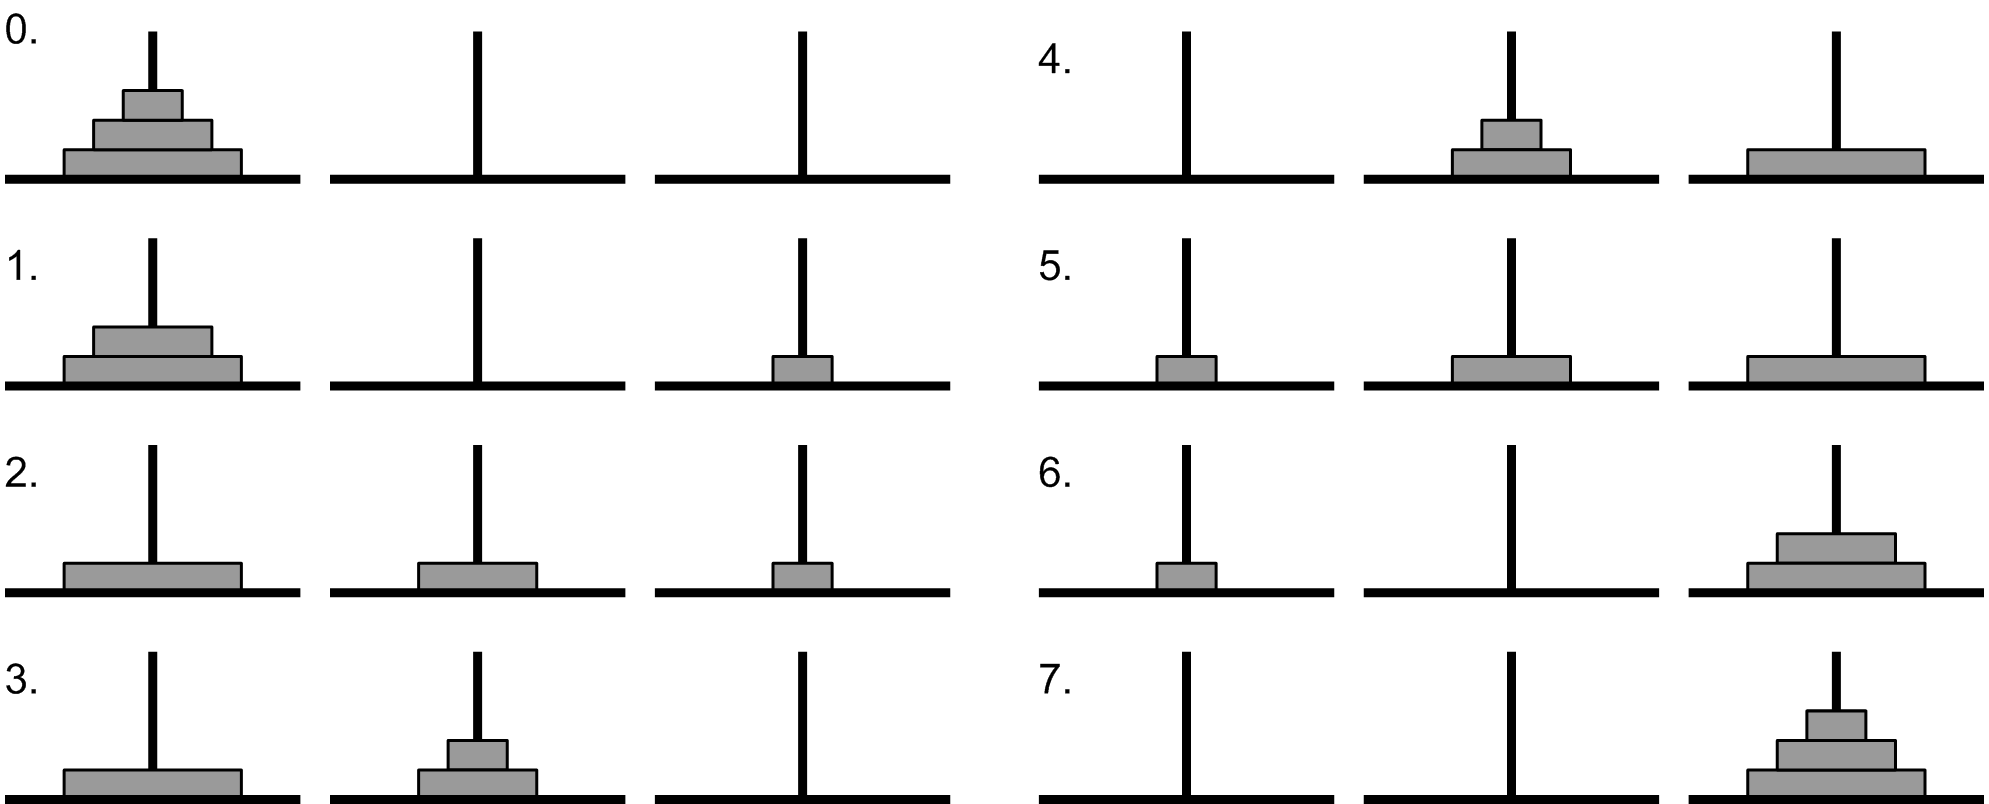
\includegraphics[scale=0.7]{hanoi.png}
	\end{center}
	\caption*{Solution to the Towers of Hanoi with 3 disks.}
	\label{fig:hanoi_solved}
\end{figure}

Solve the \textit{Tower of Hanoi} puzzle for an arbitrary number of disks, enumerating the required moves.

\solution The main insight here is that the problem involving $n$ disks can be reduced to one with $n - 1$ disks.
Labelling the rods $A$, $B$ and $C$, and the disks with numerals $1$ through $n$ (smallest to largest), our aim is to move the
entire stack from $A$ to $C$. If we can solve the problem with $n - 1$ disks, all we have to do is to move the topmost $n - 1$ disks
from $A$ to $B$, move the remaining disk on $A$ to $C$, and again move the $n - 1$ disks on $B$ to $C$. The base case for this
recursive solution is moving $1$ disk, which is trivial.

Clearly, if the problem with $n$ disks takes $k_n$ number of moves, the problem with $n + 1$ moves will take $k_n + 1 + k_n = 2k_n + 1$ moves.
For the base case with one disk, $k_1 = 1$. With this infromation, we see that the \textit{Tower of Hanoi} with $n$ disks can be solved
in exactly $2^n - 1$ moves.

\algorithm
\texttt{main (disks:Integer)}
\begin{enumerate}
	\item Call \texttt{solveHanoi(disks, "A", "C", "B")}.
	\item \textbf{Exit} 
\end{enumerate}
\vspace{5mm}
\texttt{solveHanoi (disk:Integer, source:String, destination:String, spare:String)}
\begin{enumerate}
	\item If \texttt{disk} is zero, \textbf{return}.
	\item Call \texttt{solveHanoi(disk - 1, source, spare, destination)}.
	\item Move disk number \texttt{disk} has to be moved from \texttt{source} to \texttt{destination}.
	\item Call \texttt{solveHanoi(disk - 1, spare, destination, source)}.
	\item \textbf{Return} 
\end{enumerate}

\sourcecode
\lstinputlisting{src/TowersOfHanoi.java}

\varDescription
\begin{longtable} {| >{\ttfamily}p{0.16\linewidth} | >{\ttfamily}p{0.2\linewidth}| p{0.6\linewidth} |}
\hline\multicolumn{3}{|c|}{\tt TowersOfHanoi::main(String[])} 		\\\hline
int 		&	disks	&	The number of disks in the problem \\\hline
\hline\multicolumn{3}{|c|}{\tt TowersOfHanoi::solveHanoi(int, String, String, String)} 		\\\hline
int 		&	disk	&	The current disk to be moved \\\hline
String		&	source	&	The rod from which the stack is to be moved\\\hline
String		&	destination&	The rod to which the stack is to be moved \\\hline
String		&	spare	&	The additional rod, where the remaining \texttt{n-1} disks are temporarily moved  \\\hline 
\end{longtable}

	\chapquote{``Chess is the gymnasium of the mind."}{Blaise Pascal}

\problem The {\em 8 queens puzzle} involves placing $8$ queens on an $8 \times 8$ chessboard such that no two queens
threaten each other, i.e.\ no two queens share the same rank, file or diagonal. It was first published by the chess
composer {\it Max Bezzel} in 1848. This puzzle has $92$ solutions, including reflections and rotations.
Below is one of them.
\[\chessboard[boardfontsize=25pt,
			  setpieces={Qa5, Qb3, Qc1, Qd7, Qe2, Qf8, Qg6, Qh4},
			  showmover=false,
			  arrow=to, linewidth=0.7pt, shorten=-1pt,
			  pgfstyle=straightmove]\]

The {\em n queens puzzle} is an extension of this puzzle, involving $n$ queens on an $n \times n$ chessboard.
Count the total number of solutions for the {\em n queens puzzle}, including reflections and rotations.


	
\chapquote{``In the mind's eye, a fractal is a way of seeing infinity."}{James Gleick}

\problem The \textit{Sierpinski Carpet} is a plane fractal. It can be produced iteratively by taking a solid square, dividing
it into 9 congruent squares in a 3-by-3 grid, removing the centre square, and recursively applying the same procedure on each
of the remaining squares \textit{ad infinitum}.

Display the \textit{Sierpinski Carpet} to a specified number of iterations. 

\begin{figure}[h]
	\begin{center}
		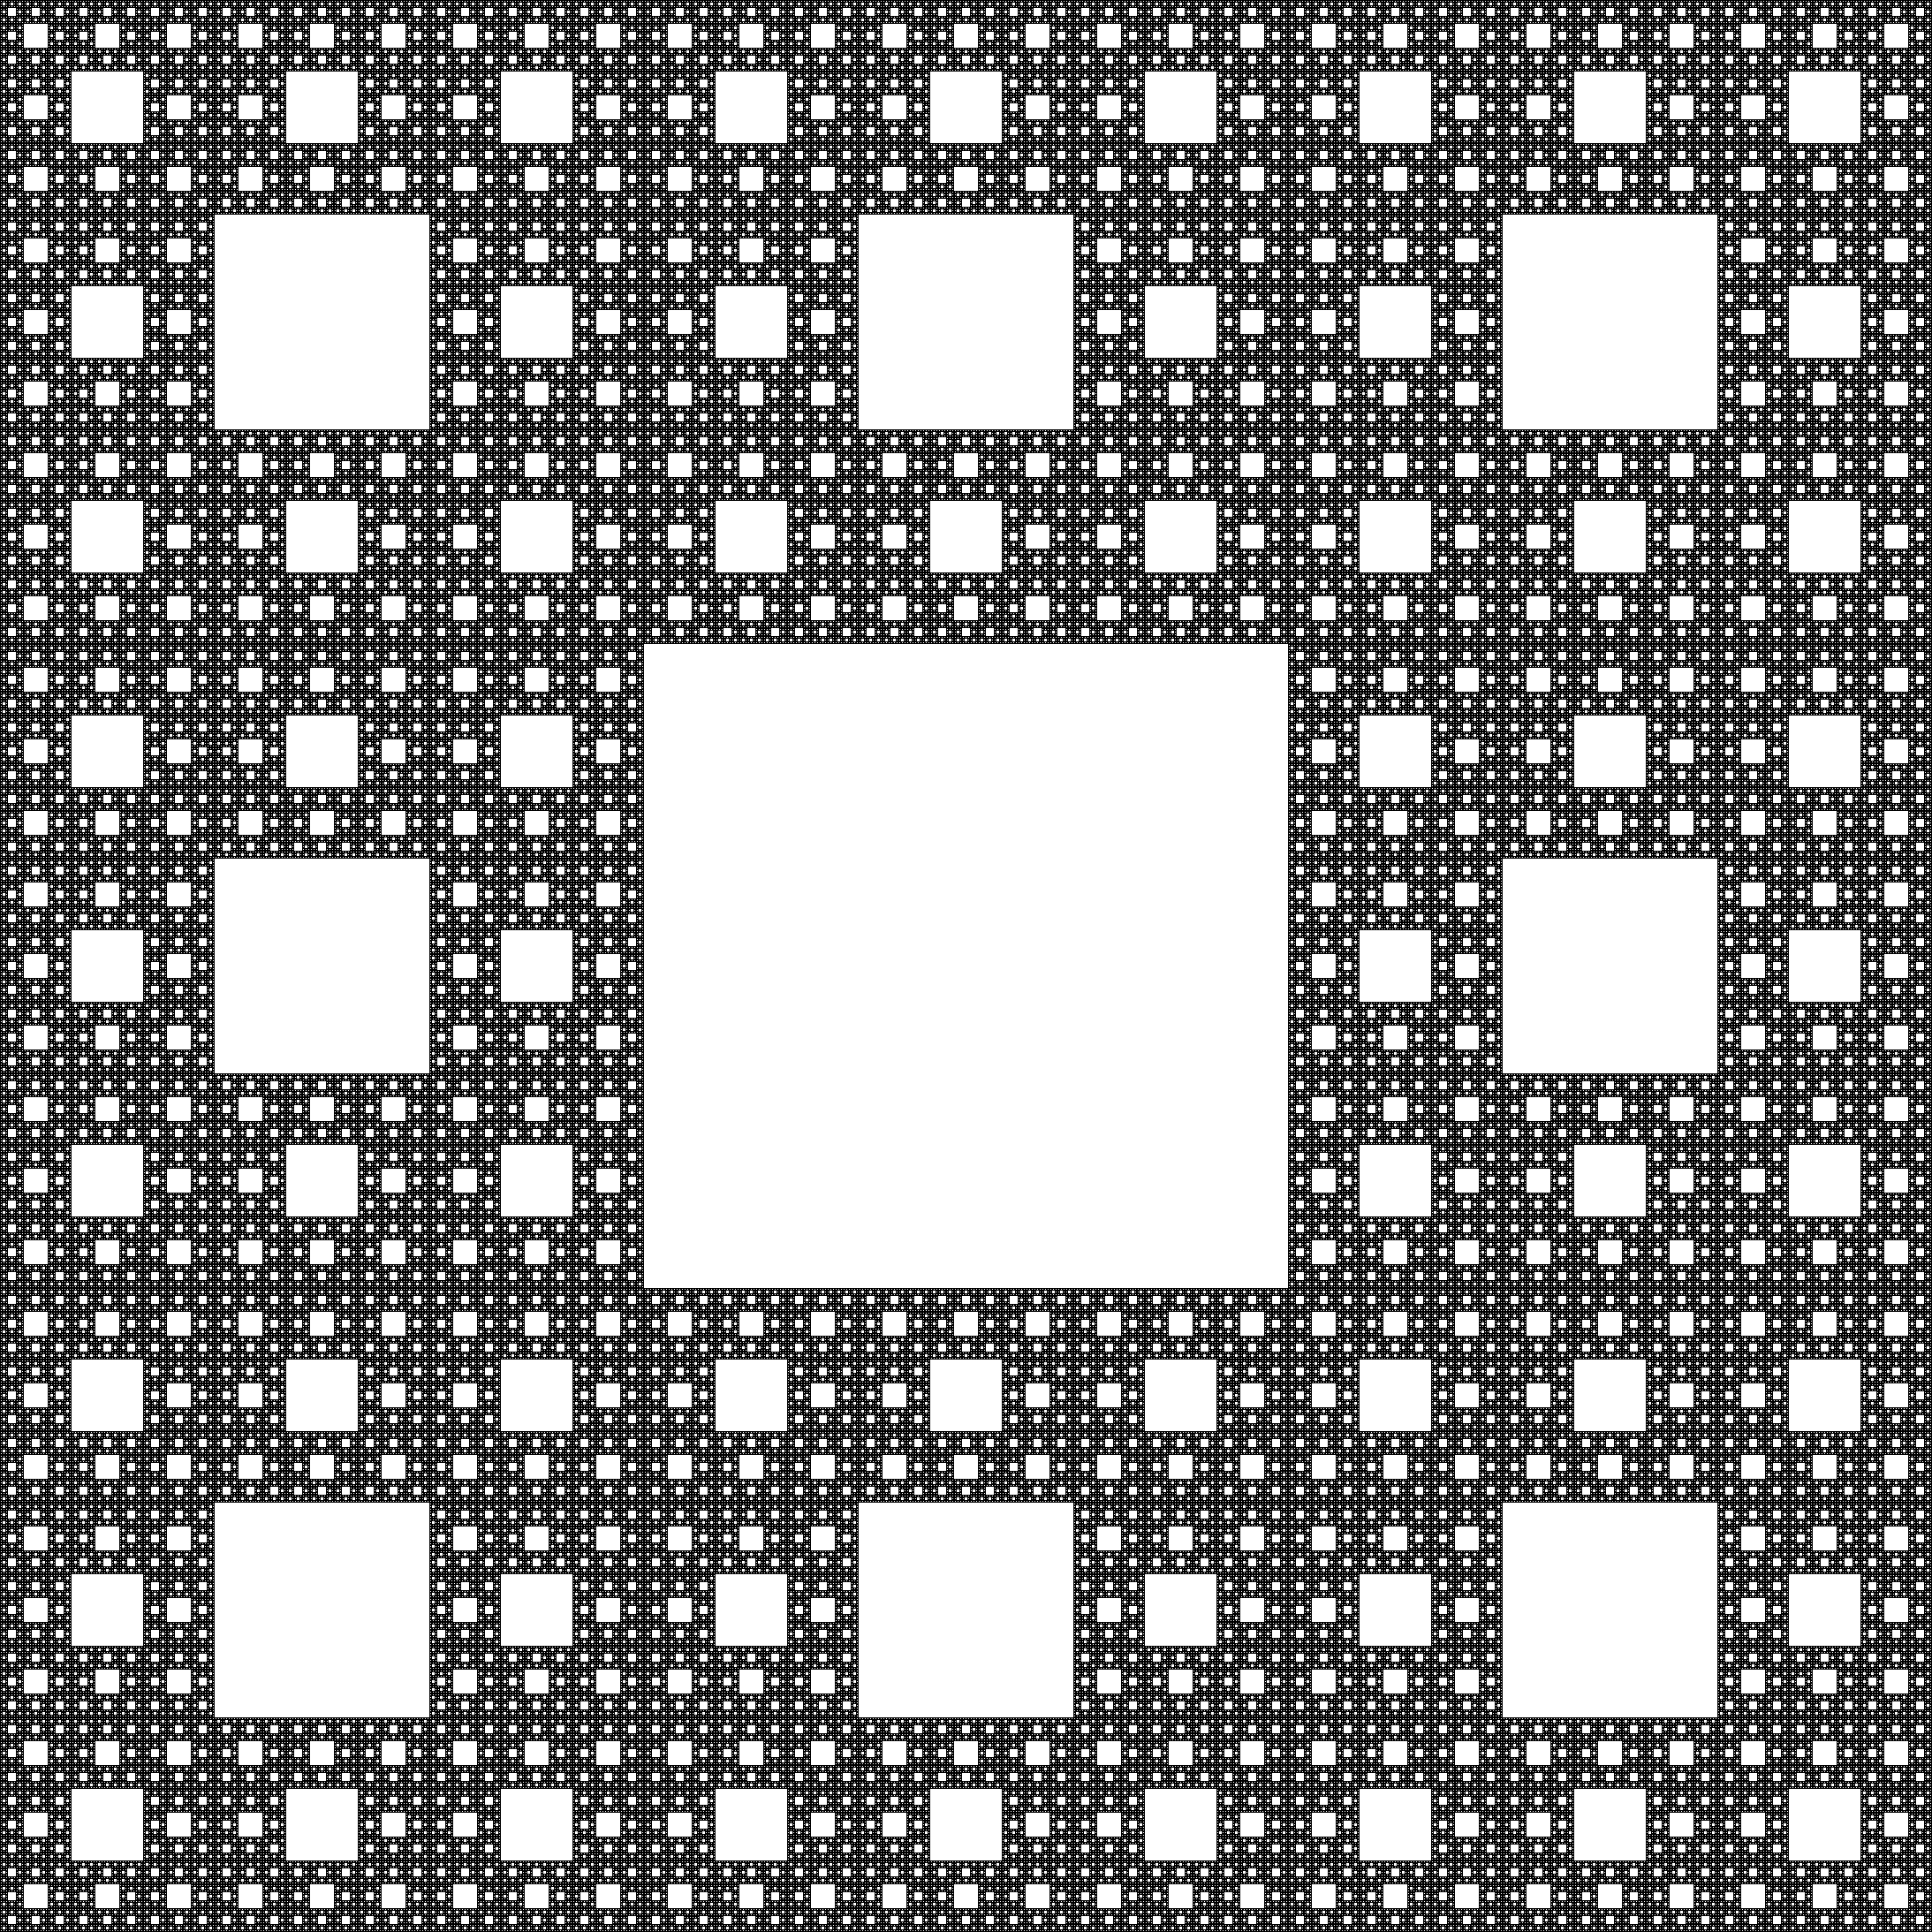
\includegraphics[scale=0.15]{sierpinski.png}
	\end{center}
	\caption*{The Sierpinski Carpet}
	\label{fig:sierpinski_carpet}
\end{figure}

\solution In an ASCII terminal, we can only display a rough representation of the \textit{Sierpinski Carpet}, a few levels deep.
A level $n$ carpet will have a width and height of $3^n$. Within this grid, every character lies either in the centre of a 3-by-3
square, in which case it is not in the carpet, or it lies on the edge, in which case it is in the carpet. If neither can be 
determined, we can scale up the search square to the next level, and repeat recursively.

Here, points in the carpet are drawn, while points not in the the carpet are left as whitespace.

\algorithm
\texttt{main (level:Integer)}
\begin{enumerate}
	\item For each pair (\texttt{i} , \texttt{j}) $\in \{0, 1, \dots, 3^n - 1\} \times \{0, 1, \dots, 3^n - 1\}$:
	\begin{enumerate}
		\item Call \texttt{isInSierpinskiCarpet(i, j)}. If it returns \texttt{true}, display a solid block
			at (\texttt{i}, \texttt{j}), otherwise, leave a blank space there.
	\end{enumerate}
	\item \textbf{Exit} 
\end{enumerate}
\vspace{5mm}
\texttt{isInSierpinskiCarpet (x:Integer, y:Integer)}
\begin{enumerate}
	\item If either of \texttt{x} or \texttt{y} is zero, the point (\texttt{x}, \texttt{y}) is on the edge of
		a square of some level. \textbf{Return} \texttt{true}.
	\item If both \texttt{x} and \texttt{y} leave a remainder of one on division by $3$, the point (\texttt{x}, \texttt{y})
		is at the centre of a square of some level. \textbf{Return} \texttt{false}.
	\item Call \texttt{isInSierpinskiCarpet(x / 3, y / 3)}, and \textbf{return} the returned value.
\end{enumerate}

\sourcecode
\lstinputlisting{src/SierpinskiCarpet.java}

\varDescription
\begin{longtable} {| >{\ttfamily}p{0.16\linewidth} | >{\ttfamily}p{0.2\linewidth}| p{0.6\linewidth} |}
\hline\multicolumn{3}{|c|}{\tt SierpinskiCarpet::main(String[])} 		\\\hline
int 		&	level		&	The depth to which to render the carpet \\\hline
int 		&	i, j		&	Counter variables, represent a point on the screen to be displayed \\\hline
\hline\multicolumn{3}{|c|}{\tt SierpinskiCarpet::isInSierpinskiCarpet(int, int)} 		\\\hline
int 		&	x, y		&	Counter variables, represent the point in question \\\hline
\end{longtable}

	
\chapquote{``Computers are useless. They can only give you answers."}{Pablo Picasso}

\problem \textit{Reverse Polish Notation (RPN)} or \textit{postfix notation} is a mathematical notation for writing arithmetic expresssions in which
operators follow their operands. Thus, as long as each operator has a fixed number of operands, the use of parentheses or rules of
precedence are no longer required to write unambiguous expressions. For example, the expression \texttt{2 3 * 3 2 \^{} 2 - *} evaluates to \texttt{42}.

Create a program capable of evaluating \textit{RPN} expressions which use the following operators.
\begin{center}
\begin{tabular}{c|l}
	{\tt +} & Addition \\
	{\tt -} & Subtraction \\
	{\tt *} & Multiplication \\
	{\tt /} & Division \\
	{\tt \^{}} & Exponentiation
\end{tabular}
\end{center}

\solution The nature of \textit{RPN} lends itself to a very simple implementation with a stack for pushing operands into as they appear
in an expression. When an operator is encountered, the required number of operands are popped from the stack, the operation is carried out,
and the result is popped back into the stack. This continued until the entire expression has been parsed, leaving only the evaluated result
in the stack.

\algorithm
\texttt{main (expression:String)}
\begin{enumerate}
	\item Call \texttt{evaluateRPNExpression(expression)} and display the returned value.
	\item \textbf{Exit} 
\end{enumerate}
\vspace{5mm}
\texttt{evaluateRPNExpression (expression:String)}
\begin{enumerate}
	\item Split \texttt{expression} along whitespace into an array of tokens. Call it \texttt{tokens}.
	\item Create a stack of floating points large enough to hold all elements in \texttt{tokens}. Call it \texttt{operandStack}.
	\item For each string \texttt{token} $\in$ \texttt{tokens}:
	\begin{enumerate}
		\item If \texttt{token} is a floating point:  \label{rpn:loopStart}
		\begin{enumerate}
			\item Push \texttt{token} onto \texttt{operandStack}.
			\item Get the next \texttt{token} from \texttt{tokens}.
			\item Jump back to (\ref{rpn:loopStart}).
		\end{enumerate}
		\item Pop an operand from \texttt{operandStack} and call it \texttt{rightOperand}. 
		\item Pop another operand from \texttt{operandStack} and call it \texttt{leftOperand}.
		\item Depending on which operator \texttt{token} represents, evaluate the operation with \texttt{token} as the operator
			and \texttt{leftOperand} and \texttt{rightOperand} as the respective operands. Call it \texttt{result}.
		\item Push \texttt{result} onto \texttt{operandStack}. 
	\end{enumerate}
	\item Pop and operand from \texttt{operandStack} and \textbf{return} it. 
\end{enumerate}

\sourcecode
\lstinputlisting{src/RPNCalculator.java}

\clearpage
\varDescription
\begin{longtable} {| >{\ttfamily}p{0.16\linewidth} | >{\ttfamily}p{0.2\linewidth}| p{0.6\linewidth} |}
\hline\multicolumn{3}{|c|}{\tt RPNCalculator} 		\\\hline
double[]	&	operandStack&	The stack of operands in order of appearance. \\\hline
int 		&	top	&	The index of the topmost element of \texttt{operandStack} \\\hline 
\hline\multicolumn{3}{|c|}{\tt RPNCalculator::main(String[])} 		\\\hline
String		&	expression&	The expression in RPN to be evaluated \\\hline
double		&	result	&	The evaluated form of \texttt{expression} \\\hline 
\hline\multicolumn{3}{|c|}{\tt RPNCalculator::evaluateRPNExpression(String)} 		\\\hline
String		&	expression&	The expression in RPN to be evaluated \\\hline
String[]	&	tokens	&	The individual tokens in \texttt{expression}, separated by whitespace \\\hline
String		&	token	&	An individual token from \texttt{tokens} \\\hline
double		&	rightOperand&	The operand to be taken on the right side of the operator \\\hline
double		&	leftOperand&	The operand to be taken on the left side of the operator \\\hline
double		&	result	&	The result on evaluating the operator \texttt{token} on \texttt{rightOperand} and \texttt{leftOperand}  \\\hline 
\hline\multicolumn{3}{|c|}{\tt RPNCalculator::pushOperand(double)} 		\\\hline
double		&	n	&	The operand to be pushed into \texttt{operandStack} \\\hline 
\hline\multicolumn{3}{|c|}{\tt RPNCalculator::isDouble(String)} 		\\\hline
String		&	n	&	The string to be tested on whether it is a floating point or not \\\hline
\end{longtable}

	
\chapquote{``Computer Science is no more about computers than astronomy is about telescopes"}{Edsger W. Dijkstra}

\problem A \textit{queue} is a linear data structure which allows storage and retrieval of elements in accordance with the
\textit{First In First Out (FIFO)} principle. Thus, elements exit a \textit{queue} in the same order they entered it.

Implement a \textit{queue} capable of holding an arbitrary number of elements of a specified type.

\solution The use of \textit{linked lists\footnote{A linked list is a linear data structure where each element is a separate object,
or \textit{node}. Each \textit{node} contains both \textit{data} and \textit{addresses} of the surrounding nodes.}} is apropriate
here. \textit{Generics} ensure that once a queue is declared with a data type, only elements of that data type can be added
to it, as opposed to merely storing \texttt{Objects}.

\algorithm
\texttt{Node<T> (item:T)}
\begin{enumerate}
	\item Copy \texttt{item} as an object variable.
	\item Declare two variables \texttt{left} and \texttt{right}, both of type \texttt{Node<T>}.
	\item \textbf{Return} the resultant object.
\end{enumerate}
\vspace{5mm}
\texttt{link (left:Node<T>, right:Node<T>)}
\begin{enumerate}
	\item Set \texttt{left->right} to \texttt{right}.
	\item Set \texttt{right->left} to \texttt{left}.
\end{enumerate}
\vspace{8mm}
\texttt{LinkedQueue<T> ()}
\begin{enumerate}
	\item Declare two constants \texttt{HEAD} and \texttt{TAIL}, both of type \texttt{Node<T>} with
		arbitrary data items.
	\item Link \texttt{TAIL} and \texttt{HEAD}.
	\item \textbf{Define} the functions:
	\begin{enumerate}
		\item \texttt{LinkedQueue<T>::enqueue(item)} 
		\item \texttt{LinkedQueue<T>::dequeue()}
		\item \texttt{LinkedQueue<T>::peek()}
		\item \texttt{LinkedQueue<T>::clear()} 
		\item \texttt{LinkedQueue<T>::isEmpty()}
		\item \texttt{LinkedQueue<T>::size()}
	\end{enumerate}
	\item \textbf{Return} the resultant object.
\end{enumerate}
\vspace{5mm}
\texttt{LinkedQueue<T>::enqueue (item:T)}
\begin{enumerate}
	\item Create a new \texttt{Node<T>}, pass it \texttt{item}, and call it \texttt{newNode}.
	\item Link \texttt{HEAD->left} and \texttt{newNode}. 
	\item Link \texttt{newNode} and \texttt{HEAD}. 
\end{enumerate}
\vspace{5mm}
\texttt{LinkedQueue<T>::dequeue ()}
\begin{enumerate}
	\item If the queue is empty, return \texttt{null}.
	\item Temporarily store the node \texttt{TAIL->right} as \texttt{lastNode}.
	\item Link \texttt{TAIL} and \texttt{lastNode->right}. 
	\item \textbf{Return} the item contained in \texttt{lastNode}. 
\end{enumerate}
\vspace{5mm}
\texttt{LinkedQueue<T>::peek ()}
\begin{enumerate}
	\item \textbf{Return} the item in the node \texttt{TAIL->right}.
\end{enumerate}
\vspace{5mm}
\texttt{LinkedQueue<T>::clear ()}
\begin{enumerate}
	\item Link \texttt{TAIL} and \texttt{HEAD}.
\end{enumerate}
\vspace{5mm}
\texttt{LinkedQueue<T>::isEmpty ()}
\begin{enumerate}
	\item If the \texttt{TAIL->right} is \texttt{HEAD}, \textbf{return} \texttt{true}, otherwise \textbf{return} \texttt{false}.
\end{enumerate}
\vspace{5mm}
\texttt{LinkedQueue<T>::size ()}
\begin{enumerate}
	\item Initialize an integer \texttt{n} to zero.
	\item Set a variable \texttt{current} to \texttt{TAIL}.
	\item While \texttt{current->right} is not \texttt{HEAD}, set \texttt{current} to \texttt{current->right} and increment \texttt{n}.
	\item \textbf{Return} \texttt{n}.
\end{enumerate}

\sourcecode
\lstinputlisting{src/Node.java}
\lstinputlisting{src/LinkedQueue.java}
\lstinputlisting{src/QueueDemo.java}

\varDescription
\begin{longtable} {| >{\ttfamily}p{0.16\linewidth} | >{\ttfamily}p{0.2\linewidth}| p{0.6\linewidth} |}
\hline\multicolumn{3}{|c|}{\tt Node<T>} 		\\\hline
T		&	item 		&	The data stored in the node \\\hline
Node<T>		&	left		&	Reference to the node to the left of \texttt{this} \\\hline
Node<T>		&	right		&	Reference to the node to the right of \texttt{this} \\\hline
\hline\multicolumn{3}{|c|}{\tt LinkedQueue<T>} 		\\\hline
Node<T>		&	HEAD		&	Special node, marks the point of entry of new data \\\hline
Node<T>		&	TAIL		&	Special node, marks the point of exit of data \\\hline
\hline\multicolumn{3}{|c|}{\tt LinkedQueue<T>::enqueue(T)} 		\\\hline
T		&	item 		&	The data to be enqueued \\\hline
\hline\multicolumn{3}{|c|}{\tt LinkedQueue<T>::dequeue()} 		\\\hline
Node<T>		&	lastNode	&	The node containing the data to be dequeued \\\hline
\hline\multicolumn{3}{|c|}{\tt LinkedQueue<T>::size()} 		\\\hline
int 		&	n		&	Stores the number of elements in the queue \\\hline
\hline\multicolumn{3}{|c|}{\tt LinkedQueue<T>::toString()} 		\\\hline
String[]	&	elements	&	Temporary array, stores the string representations of the data items in the queue \\\hline
int 		&	n		&	Counter variable \\\hline
\end{longtable}


	
\chapquote{``A good way to have good ideas is by being unoriginal."}{Bram Cohen}

\problem A \textit{double ended queue}, or \textit{DEqueue} is a linear data structure which allows the insertion
and deletion of data items from both the front and rear.

Implement a \textit{double ended queue} capable of holding an arbitrary number of elements of a specified type.

\solution 
This problem can be solved by extending the funcitonality of the \textit{queue} defined in the previous problem. The algorithms
for insertion and deletion at one end mirror those for the other.

\algorithm
\texttt{LinkedDEQueue<T> ()}
\begin{enumerate}
	\item Call the constructor of the superclass \texttt{LinkedQueue}.
	\item \textbf{Define} the functions:
	\begin{enumerate}
		\item \texttt{LinkedDEQueue<T>::enqueueRear(item)} 
		\item \texttt{LinkedDEQueue<T>::dequeueFront()}
	\end{enumerate}
	\item \textbf{Return} the resultant object.
\end{enumerate}
\vspace{5mm}
\texttt{LinkedDEQueue<T>::enqueueRear (item:T)}
\begin{enumerate}
	\item Create a new \texttt{Node<T>}, pass it \texttt{item}, and call it \texttt{newNode}.
	\item Link \texttt{newNode} and \texttt{TAIL->right}. 
	\item Link \texttt{TAIL} and \texttt{newNode}. 
\end{enumerate}
\vspace{5mm}
\texttt{LinkedDEQueue<T>::dequeueFront ()}
\begin{enumerate}
	\item If the queue is empty, return \texttt{null}.
	\item Temporarily store the node \texttt{HEAD->left} as \texttt{firstNode}.
	\item Link \texttt{firstNode->left} and \texttt{HEAD} . 
	\item \textbf{Return} the item contained in \texttt{firstNode}. 
\end{enumerate}

\clearpage
\sourcecode
\lstinputlisting{src/LinkedDEQueue.java}
\lstinputlisting{src/DEQueueDemo.java}

\varDescription
\begin{longtable} {| >{\ttfamily}p{0.16\linewidth} | >{\ttfamily}p{0.2\linewidth}| p{0.6\linewidth} |}
\hline\multicolumn{3}{|c|}{\tt LinkedDEQueue<T>::enqueueRear(T)} 		\\\hline
T		&	item 		&	The data to be enqueued \\\hline
\hline\multicolumn{3}{|c|}{\tt LinkedDEQueue<T>::dequeueFront()} 		\\\hline
Node<T>		&	firstNode	&	The node containing the data to be dequeued \\\hline
\end{longtable}

	
\chapquote{``You can't trust code that you did not totally create yourself."}{Ken Thompson}

\problem Arrange the words in a given sentence of input in alphabetical order.

\textit{(Ignore case, duplicated words.)} 

\solution This problem can be solved using a data structure called a \textit{binary tree}.\\

A \textit{binary tree} consists of multiples \textit{nodes}, each of which holds a data item. Ideally, 
these items can be \textit{ordered}, i.e., there is a way to compare them, using a value called a \textit{key}.
Each node is connected to two nodes below it --- the \textit{left child} and the \textit{right child}. The left child
has  lower \textit{key}, while the right child has a higher \textit{key} than the parent node. The node at the top 
of a given binary tree is called its \textit{root}.

Binary trees have a nice recursive form, in that the left and right children of the root can be regarded as roots of 
individual binary trees --- the \textit{left} and \textit{right} \textit{subtrees} of the root. This makes it easy to
write recursive algorithms for searching, inserting, and deleting nodes from a binary tree.

Searching and insertion in a binary tree containing $n$ nodes have an average time complexity $O(\log{n})$.

\algorithm
\texttt{TreeNode<T> (item:T)}
\begin{enumerate}
	\item Copy \texttt{item} as an object variable.
	\item Declare two variables \texttt{left} and \texttt{right}, both of type \texttt{Node<T>}.
	\item \textbf{Return} the resultant object.
\end{enumerate}
\vspace{8mm}
\texttt{BinaryTree<T> (root:TreeNode<T>)}
\begin{enumerate}
	\item Copy \texttt{root} as an object variable.
	\item \textbf{Define} the functions:
	\begin{enumerate}
		\item \texttt{BinaryTree<T>::contains(item)} 
		\item \texttt{BinaryTree<T>::search(item)} 
		\item \texttt{BinaryTree<T>::add(item)} 
	\end{enumerate}
	\item \textbf{Return} the resultant object.
\end{enumerate}
\vspace{5mm}
\texttt{BinaryTree<T>::contains (item:T)}
\begin{enumerate}
	\item If \texttt{this->search(item)} returns a non-null object, \textbf{return} \texttt{true}, otherwise
		\textbf{return} \texttt{false}.
\end{enumerate}
\vspace{5mm}
\texttt{BinaryTree<T>::search (item:T)}
\begin{enumerate}
	\item \textbf{Return} \texttt{search(this->root, item)}
\end{enumerate}
\vspace{5mm}
\texttt{BinaryTree<T>::add (item:T)}
\begin{enumerate}
	\item Set \texttt{this->root} to the \texttt{TreeNode} returned by \texttt{add(this->root, item)}.
\end{enumerate}
\vspace{5mm}
\texttt{search (root:TreeNode<T>, item:T)} 
\begin{enumerate}
	\item If \texttt{item} $<$ \texttt{root->item}, \textbf{return} \texttt{search(root->left, item)}
	\item If \texttt{item} $>$ \texttt{root->item}, \textbf{return} \texttt{search(root->right, item)}
	\item \textbf{Return} \texttt{root}
\end{enumerate}
\vspace{5mm}
\texttt{add (root:TreeNode<T>, item:T)}
\begin{enumerate}
	\item If \texttt{root} is \texttt{null}, set it to a new \texttt{TreeNode<T>} containing \texttt{item} and
		\textbf{return} \texttt{root}.
	\item If \texttt{item} $<$ \texttt{root->item}, set \texttt{root->left} to \texttt{add(root->left, item)}.
	\item If \texttt{item} $>$ \texttt{root->item}, set \texttt{root->right} to \texttt{add(root->right, item)}.
	\item \textbf{Return} \texttt{root}
\end{enumerate}
\vspace{5mm}
\texttt{traverseInOrder (node:TreeNode<T>)}
\begin{enumerate}
	\item If \texttt{node} is \texttt{null}, \textbf{return} an empty string.
	\item \textbf{Return} \texttt{traverseInOrder(node->left)} \texttt{+} \texttt{node} \texttt{+} \texttt{traverseInOrder(node->right)} 
		\textit{(with spacing as necessary)}.
\end{enumerate}

\sourcecode
\lstinputlisting{src/TreeNode.java}
\lstinputlisting{src/BinaryTree.java}
\lstinputlisting{src/BinaryTreeDemo.java}

\varDescription
\begin{longtable} {| >{\ttfamily}p{0.16\linewidth} | >{\ttfamily}p{0.2\linewidth}| p{0.6\linewidth} |}
\hline\multicolumn{3}{|c|}{\tt TreeNode<T>} 		\\\hline
T		&	item 		&	The data stored in the node \\\hline
TreeNode<T>	&	left		&	Reference to the left child of \texttt{this} \\\hline
TreeNode<T>	&	right		&	Reference to the right child of \texttt{this} \\\hline
\hline\multicolumn{3}{|c|}{\tt BinaryTree<T>} 		\\\hline
TreeNode<T>	&	root		&	The root node of the binary tree \\\hline
\hline\multicolumn{3}{|c|}{\tt BinaryTree<T>::contains(T)} 		\\\hline
T		&	item 		&	The item to check for	\\\hline	
\hline\multicolumn{3}{|c|}{\tt BinaryTree<T>::search(T)} 		\\\hline
T		&	item 		&	The item to search for	\\\hline	
\hline\multicolumn{3}{|c|}{\tt BinaryTree<T>::add(T)} 		\\\hline
T		&	item 		&	The item to be added	\\\hline
\hline\multicolumn{3}{|c|}{\tt BinaryTree<T>::search(TreeNode<T>, T)} 		\\\hline
TreeNode<T>	&	root		&	The current node being checked \\\hline
T		&	item 		&	The item to search for	\\\hline
\hline\multicolumn{3}{|c|}{\tt BinaryTree<T>::add(TreeNode<T>, T)} 		\\\hline
TreeNode	&	root		&	The current node being compared 	\\\hline
T		&	item 		&	The item to be added	\\\hline
\end{longtable}

	
\chapquote{``One should always play fairly when one has the winning cards."}{Oscar Wilde}

\problem

\solution

\algorithm

\sourcecode
\lstinputlisting{src/Suit.java}
\lstinputlisting{src/Rank.java}
\lstinputlisting{src/Card.java}
\lstinputlisting{src/Deck.java}
\lstinputlisting{src/DeckDemo.java}

\varDescription

	
\chapquote{``Code never lies, comments sometimes do."}{Ron Jeffries}

\problem Remove all comments from given source code.

\solution
Java comments can be classified into two broad types --- single line comments beginning with the sequence `\texttt{//}' and
ending with a newline, and multiple line comment beginning with the sequence `\texttt{/*}' and ennding with the sequence `\texttt{*/}'.
Care must be taken to ignore such sequences within quotes \textit{both single and double}, as well as within other comments.
Escape sequences also have to be dealt with.

While parsing the given source code character by character, it becomes necessary to keep track of a \textit{state variable}. This
will store information about what is currently being parsed, and different sets of checks are executed accordingly. Java \textit{enums}, 
or \textit{enumerated lists}, are ideal for this purpose.

\algorithm
\texttt{main (filename:String)}
\begin{enumerate}
	\item Create a \texttt{ReadSourceFile} object called \texttt{s}, and pass it \texttt{filename} and a buffer size of $10$.
	\item Declare a state variable called \texttt{currentState}, and set it to \texttt{SOURCE}.
	\item Declare a character called \texttt{matchingQuotes}, and set it to a black space.
	\item \textbf{While} \texttt{s->hasNextChar()}: \label{rc:while}
	\begin{enumerate}
		\item Store the character returned by \texttt{s->getChar()} as \texttt{c}.
		\item If \texttt{c} is a backslash, display it, get another character from \texttt{s->getChar()},
			display that, and jump to (\ref{rc:while}).
		\item If \texttt{currentState} is \texttt{SOURCE}:
		\begin{enumerate}
			\item If \texttt{c} is a quotation mark, set \texttt{currentState} to \texttt{QUOTES}, set \texttt{matchingQuotes} to
				\texttt{c}. Display \texttt{c} and jump to (\ref{rc:while}).
			\item If \texttt{c} is a forward slash, get another character called \texttt{n} from \texttt{s->getChar()}.
			\begin{enumerate}
				\item If \texttt{n} is an asterisk, set \texttt{currentState} to \texttt{MULTIPLE\_LINE\_COMMENT}.
				\item If \texttt{n} ia another forward slash, set \texttt{currentState} to \texttt{SIMGLE\_LINE\_COMMENT}.
				\item If none of the above, call \texttt{s->putChar(n)}, display \texttt{c} and jump to (\ref{rc:while}).
			\end{enumerate}
			\item If none of the above, display \texttt{c} and jump to (\ref{rc:while}).
		\end{enumerate}
		\item If \texttt{currentState} is \texttt{SIMGLE\_LINE\_COMMENT} and \texttt{c} is a newline, set \texttt{currentState} to
			\texttt{SOURCE}, display \texttt{c} and jump to (\ref{rc:while}).
		\item If \texttt{currentState} is \texttt{MULTIPLE\_LINE\_COMMENT} and \texttt{c} is an asterisk:
		\begin{enumerate}
			\item Get another character called \texttt{n} from \texttt{s->getChar()}.
			\item If \texttt{n} is a forward slash, set \texttt{currentState} to \texttt{SOURCE}.
			\item Jump to (\ref{rc:while}).
		\end{enumerate}
		\item If \texttt{currentState} is \texttt{QUOTES} and \texttt{c} is equal to \texttt{matchingQuotes}, set \texttt{currentState}
			to \texttt{SOURCE}, \texttt{matchingQuotes} to an blank space. Display \texttt{c} and jump to (\ref{rc:while}).
		\item If none of the above, display \texttt{c}.
	\end{enumerate}
\end{enumerate}
\vspace{8mm}
\texttt{ReadSourceFile (filename:String, bufferSize:integer)}
\begin{enumerate}
	\item Initialize a new \texttt{FileReader} \textit{unbuffered} called \texttt{fileReader} and pass it \texttt{filename}.
	\item Create a simple \textit{buffer} of integers, implemented using a stack.
		\textit{This will store characters, but the \texttt{char} data type cannot store special characters, such as the character
			which indicates the end of a file.}
	\item \textbf{Define} the functions:
	\begin{enumerate}
		\item \texttt{ReadSourceFile::hasNextChar()}
		\item \texttt{ReadSourceFile::getChar()}
		\item \texttt{ReadSourceFile::putChar(c)}
	\end{enumerate}
	\item \textbf{Return} the resultant object.
\end{enumerate}
\vspace{5mm}
\texttt{ReadSourceFile::hasNextChar ()} 
\begin{enumerate}
	\item Read a new character from \texttt{fileReader}, and call it \texttt{c}.
	\item If \texttt{c} is equal to $-1$, \textbf{return} \texttt{false}.
	\item Call \texttt{this->putChar(c)}
	\item \textbf{Return} \texttt{true}
\end{enumerate}
\vspace{5mm}
\texttt{ReadSourceFile::getChar ()}
\begin{enumerate}
	\item If the buffer has some characters, pop one off and \textbf{return} it.
	\item Read a character from \texttt{fileReader} and \textbf{return} it.
\end{enumerate}
\vspace{5mm}
\texttt{ReadSourceFile::putChar (c:Integer)}
\begin{enumerate}
	\item If the buffer has space, push \texttt{c} onto it and \textbf{return} \texttt{true}. Otherwise, 
		\textbf{return} \texttt{false}.
\end{enumerate}

\clearpage
\sourcecode
\lstinputlisting{src/State.java}
\lstinputlisting{src/ReadSourceFile.java}
\lstinputlisting{src/RemoveComments.java}

\varDescription
\begin{longtable} {| >{\ttfamily}p{0.16\linewidth} | >{\ttfamily}p{0.2\linewidth}| p{0.6\linewidth} |}
\hline\multicolumn{3}{|c|}{\tt ReadSourceFile} 		\\\hline
String		&	filename	&	The file containing the source code to be read \\\hline
int[]		&	buffer		&	The stack of characters read from the file \\\hline
int 		&	top		&	The index of the character at the top of the buffer \\\hline
\hline\multicolumn{3}{|c|}{\tt RemoveComments::main(String[])} 		\\\hline
ReadSource\newline
	File	&	s		&	The source file reader \\\hline
State		&	currentState	&	Indicates the type of code currently being parsed \\\hline
char		&	matchingQuotes	&	Indicates the type of ending quote which pairs with the opening quote,
						if currently inside a string in the source code \\\hline
char		&	c, n		&	Stores the current and next characters in the source code being parsed \\\hline
\end{longtable}

	
\chapquote{``A program that produces incorrect results twice as fast is infinitely slower."}{John Ousterhout}

\problem Compare the runtimes of the following sorting algorithms --- \textit{bubble sort}, \textit{insertion sort} and \textit{quicksort}.

\solution \textit{Bubble sort} is a sorting algorithm which repeatedly steps through an unsorted list, compares adjacent elements and
swaps them if they are in the wrong order. It has an average time complexity of $O(n^2)$.

\textit{Insertion sort} is a sorting algorithm which builds a sorted list one element at a time by repeatedly selecting an unsorted
element and inserting it into the correct position in the sorted portion. It too has an average time complexity of $O(n^2)$

\textit{Quicksort} is a \textit{divide and conquer} sorting algorithm which splits an unsorted list along a pivot, with elements
less than it shifted before and elements greater than it shifted after. The two halves are then sorted recursively. This algorithm has
an average time complexity of $O(n \log{n})$.

Each of these algorithms have different strengths and weaknesses. \textit{Insertion sort} and \textit{bubble sort} perform progressively slower than
\textit{quicksort} on long lists with a large spread of randomly shuffled numbers. On the other hand, \textit{insertion sort} performs faster than
\textit{bubble sort}, which in turn performs faster than quicksort on shorter lists with randomly shuffled numbers. Again, \textit{bubble sort} 
performs faster than \textit{insertion sort}, which performs significantly faster on long lists with a small spread of numbers, i.e., almost sorted
lists.\\

\algorithm
\texttt{BubbleSorter::sort (a:Integer[])} 
\begin{enumerate}
	\item Initialize an integer \texttt{right} to the length of \texttt{a}.
	\item Initialize a boolean \texttt{swapped} to \texttt{true}.
	\item \textbf{While} \texttt{swapped}:
	\begin{enumerate}
		\item Set \texttt{swapped} to \texttt{false}
		\item For \texttt{i} $ \in \{1, 2, \dots, right - 1\}$:
		\begin{enumerate}
			\item If \texttt{a[i - 1]} $ > $ \texttt{a[i]}:
			\begin{enumerate}
				\item Swap the elements in \texttt{a} at indices \texttt{i-1} and \texttt{i}.
				\item Set \texttt{swapped} to \texttt{true}.
			\end{enumerate}
		\end{enumerate}
		\item Decrement \texttt{right}.
	\end{enumerate}
\end{enumerate}
\vspace{8mm}
\texttt{InsertionSorter::sort (a:Integer[])}
\begin{enumerate}
	\item Let $n$ be thenumber of elements in \texttt{a}.
	\item For \texttt{i} $ \in \{1, 2, \dots, n - 1\}$:
	\begin{enumerate}
		\item Set an integer \texttt{k} to \texttt{a[i]}.
		\item Set an integer \texttt{j}	to \texttt{i - 1}.
		\item \textbf{While} (\texttt{j} $ \geq 0$) and (\texttt{a[j]} $ > $ \texttt{k}):
		\begin{enumerate}
			\item Set \texttt{a[j + 1]} to \texttt{a[j]}.
			\item Decrement \texttt{j}.
		\end{enumerate}
		\item Set \texttt{a[j + 1]} to \texttt{k}.
	\end{enumerate}
\end{enumerate}
\vspace{8mm}
\texttt{QuickSorter::sort (a:Integer[])}
\begin{enumerate}
	\item Let \texttt{l} be the number of elements in \texttt{a}.
	\item Call \texttt{this->sort(a, 0, l - 1)}
\end{enumerate}
\vspace{5mm}
\texttt{QuickSorter::sort (a:Integer[], lo:Integer, hi:Integer)}
\begin{enumerate}
	\item If \texttt{hi} $ \leq $ \texttt{lo}, \textbf{return}.
	\item Call \texttt{this->partition(a, lo, hi)}, and store the returned integer as \texttt{pivot}.
	\item Call \texttt{this->sort(a, lo, pivot - 1)}
	\item Call \texttt{this->sort(a, pivot + 1, hi)} 
\end{enumerate}
\vspace{5mm}
\texttt{QuickSorter::partition (a:Integer[], lo:Integer, hi:Integer)} 
\begin{enumerate}
	\item Set an integer \texttt{pivotValue} to \texttt{a[hi]}.
	\item Set an integer \texttt{pivot} to \texttt{lo - 1}.
	\item For \texttt{i} $ \in \{$\texttt{lo}$, $\texttt{lo + 1}$, \dots, $\texttt{hi - 1} $\}$:
	\begin{enumerate}
		\item If \texttt{a[i]} $ \leq $ \texttt{pivotValue}:
		\begin{enumerate}
			\item Increment \texttt{pivot}.
			\item Swap the elements in \texttt{a} at indices \texttt{i} and \texttt{pivot}.
		\end{enumerate}
	\end{enumerate}
	\item Increment \texttt{pivot}.
	\item Swap the elements in \texttt{a} at indices \texttt{i} and \texttt{pivot}.
	\item \textbf{Return} \texttt{pivot}
\end{enumerate}

\clearpage
\sourcecode
\lstinputlisting{src/IntegerArraySorter.java}
\lstinputlisting{src/BubbleSorter.java}
\lstinputlisting{src/InsertionSorter.java}
\lstinputlisting{src/QuickSorter.java}
\lstinputlisting{src/SortCompare.java}

\clearpage
\varDescription
\begin{longtable} {| >{\ttfamily}p{0.16\linewidth} | >{\ttfamily}p{0.2\linewidth}| p{0.6\linewidth} |}
\hline\multicolumn{3}{|c|}{\tt IntegerArraySorter::sort(int[])} 		\\\hline
int[]		&	a		&	The array whose elements are to be sorted \\\hline
\hline\multicolumn{3}{|c|}{\tt IntegerArraySorter::swap(int[], int, int)} 		\\\hline
int[]		&	a		&	The array whose elements are to be swapped \\\hline
int 		&	i, j 		&	The indices of the elements to be swapped \\\hline
\hline\multicolumn{3}{|c|}{\tt BubbleSorter::sort(int[])} 		\\\hline
int[]		&	a		&	The array whose elements are to be sorted \\\hline
int 		&	right, 	i	&	Counter variables	\\\hline
boolean 	&	swapped		&	Keeps track of whether any swaps were performed in the current iteration \\\hline
\hline\multicolumn{3}{|c|}{\tt InsertionSorter::sort(int[])} 		\\\hline
int[]		&	a		&	The array whose elements are to be sorted \\\hline
int 		&	i, j		&	Counter variables \\\hline
int 		&	k		&	The element to be inserted \\\hline
\hline\multicolumn{3}{|c|}{\tt QuickSorter::sort(int[])} 		\\\hline
int[]		&	a		&	The array whose elements are to be sorted \\\hline
\hline\multicolumn{3}{|c|}{\tt QuickSorter::sort(int[], int, int)} 		\\\hline
int[]		&	a		&	The array whose elements are to be sorted \\\hline
int 		&	lo, hi		&	The lower and upper indices of the unsorted list \\\hline
int 		&	pivot		&	The index of the value about which the list is partitioned \\\hline
\hline\multicolumn{3}{|c|}{\tt QuickSorter::partition(int[], int, int)} 		\\\hline
int[]		&	a		&	The array whose elements are to be sorted \\\hline
int 		&	lo, hi		&	The lower and upper indices of the unsorted list \\\hline
int 		&	pivotValue	&	The value about which the list is partitioned \\\hline
int 		&	pivot		&	The index of the value about which the list is partitioned \\\hline
int 		&	i		&	Counter variable \\\hline
\end{longtable}

	 
\chapquote{``Design is choosing how you will fail."}{Ron Fein}

\problem

\solution

\tikzstyle{vertex}=[draw]
\tikzstyle{edge}=[draw, -latex, >=stealth, line width=0.2mm]

\begin{figure}[htpb]
\begin{center}
\begin{tikzpicture}[scale=0.75, auto]
	\foreach \pos/\name in {{(6,4)/Circle}, {(3,4)/Triangle}, {(0,4)/Rectangle}, {(0,2)/Square},
				{(10.5,4)/Sphere}, {(15.5,4)/Cuboid}, {(15.5,2)}/Cube, {(8,-0.5)/LineSegment}}
		\node[vertex] (\name) at \pos {\texttt{\name}};
	\foreach \pos/\name in {{(8,10)/Shape}, {(3,7)/Shape2D}, {(13,7)/Shape3D}, {(8,1)/Scalable}}
		\node[vertex] (\name) at \pos {\textit{\name}};
	\foreach \source/\dest in {Shape/Shape2D, Shape/Shape3D, Shape2D/Circle, Shape2D/Triangle,
				   Shape2D/Rectangle, Rectangle/Square, Shape3D/Sphere, Shape3D/Cuboid, Cuboid/Cube,
				   Scalable/LineSegment, Scalable/Circle, Scalable/Rectangle, Scalable/Triangle,
				   Scalable/Sphere, Scalable/Cuboid}
		\path[edge] (\source) -> (\dest);
\end{tikzpicture}
\end{center}
\label{fig:shape_tree}
\end{figure}

\algorithm

\sourcecode
\lstinputlisting{src/Scalable.java}
\lstinputlisting{src/LineSegment.java}
\lstinputlisting{src/Shape.java}
\lstinputlisting{src/Shape2D.java}
\lstinputlisting{src/Circle.java}
\lstinputlisting{src/Triangle.java}
\lstinputlisting{src/Rectangle.java}
\lstinputlisting{src/Square.java}
\lstinputlisting{src/Shape3D.java}
\lstinputlisting{src/Sphere.java}
\lstinputlisting{src/Cuboid.java}
\lstinputlisting{src/Cube.java}

\varDescription

	\include{tex/numbertowords}
	
\chapquote{``Please, Oh please, publish me in your collection of self-referential sentences!"}{Douglas Hofstadter}

\problem A \textit{quine} is a non-empty computer program which takes no input and produces a copy of its own source code as its only
output.

Write a \textit{quine} in \textit{Java}.


\textit{(Note that a program which finds its source code file and displays it is not considered a \textit{quine}, since it takes a file as input.)}

\solution
\begin{figure}[h]
	\begin{center}
		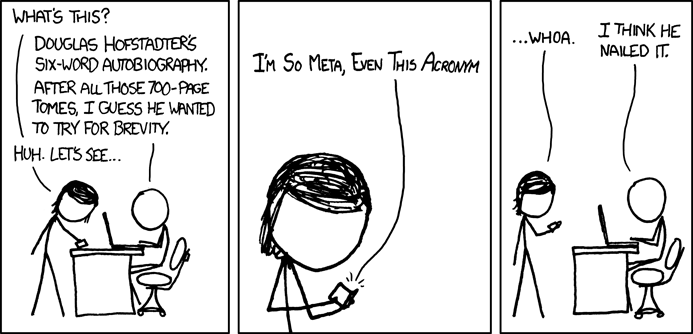
\includegraphics[scale=0.5]{hofstadter.png}
	\end{center}
	\caption*{Hofstadter (\texttt{xkcd.com/917})}
	\label{fig:xkcd_hofstadter}
\end{figure}

The name \textit{quine} was coined by \textit{Douglas Hofstadter} in his brilliant book \textit{G\"odel, Escher, Bach: An Eternal Golden Braid}, in
honour of the philosopher \textit{Willard Van Orman Quine}, who extensively studied indirect self reference, in particular the following
statement known as \textit{Quine's paradox}.
\begin{quote}
	``Yields falsehood when preceded by its quotation" yields falsehood when preceded by its quotation.
\end{quote}

Although writing a \textit{quine} in \textit{Java} seems impossible at first glance, it can be shown that \textit{quines}
exist in any \textit{Turing complete} programming language.

We might start off by writing the following code.
\lstinputlisting{QuineA.java}
A problem arises --- what can we write in place of \texttt{???} ? This part of the string must contain the entire string itself.
Is this possible without the string being infinitely long?

The problem is that the string we seek must contain the characters to be printed, and also be able to be used to print itself.
The following code snippet illustrates this.
\lstinputlisting{QuineB.java}
What can replace \texttt{???} so that the entirety of line 1 is displayed?

A solution is as follows.
\lstinputlisting{QuineC.java}

We can now use this template to move the entirety of the code into the string, including the print statement itself. This leads to another problem
--- double quotes are now inside double quotes, and must be escaped (\texttt{\textbackslash"}). However, the backslashes themselves will not appear
in the output. This can be solved by using the ASCII value for an double quote, which is \texttt{34}, in place of an escaped double quote.
Discarding newlines and delcaring the string \texttt{s} as a global variable at the very end of the program minimizes the amount of code
considerably.

The result is the following \textit{quine}.

\lstinputlisting{src/Quine.java}

\varDescription
\begin{longtable} {| >{\ttfamily}p{0.16\linewidth} | >{\ttfamily}p{0.2\linewidth}| p{0.6\linewidth} |}
\hline\multicolumn{3}{|c|}{\tt Quine} 		\\\hline
String		&	s		&	Stores the entire source code of the program \\\hline
\hline\multicolumn{3}{|c|}{\tt Quine::main()} 		\\\hline
char		&	q		&	Stores a double quote	\\\hline
\end{longtable}


	
\thispagestyle{empty}\addtocounter{page}{-1}
\hspace{0pt}
\vfill
\begin{center}
This project was compiled with \XeLaTeX .\\
\vspace{5mm}
All files involved in the making of this project can be found at
{\tt https://github.com/sahasatvik/Computer-Project/tree/master/ISC}
\vfill
{\fontsize{24}{24}\JennaSue Satvik Saha}\\
{\fontsize{10}{8}\tt sahasatvik@gmail.com}\\
\vspace{-1mm}
{\fontsize{10}{8}\tt https://sahasatvik.github.io}
\end{center}
\hspace{0pt}

\end{document}
\end
